% main.tex -- Rival-conditioned evidence attention (RCEA): paper draft. Methods and protocol written before the test
% results (8 November 2026); results of the main experiments and the ResNet-50 study filled in from the digest on
% 9 November 2026; the secondary experiments, finished on Kaggle the same night, filled in from the merged digest
% (9 November 2026, 06:00 UTC).
% Pure ASCII source. Tables are generated by scripts/make_tables.py (paper/generated/tab_*.tex) and figures by
% scripts/make_figures.py (paper/figures/fig_*.pdf); a missing input prints a visible "pending" box instead.
% \pending{...} marks every statement that can only be written from the results, and names its source.
% Build: cd paper && latexmk -pdf -interaction=nonstopmode -halt-on-error main.tex
\documentclass[11pt,a4paper]{article}

% Latin Modern with T1 when installed (Debian: the lmodern package); otherwise the scalable OT1 Computer Modern,
% so that microtype never meets a bitmap font
\IfFileExists{lmodern.sty}{\usepackage[T1]{fontenc}\usepackage{lmodern}}{}
\usepackage[utf8]{inputenc}
\usepackage[a4paper,textwidth=16cm,top=2.5cm,bottom=2.6cm]{geometry}
\usepackage{amsmath,amssymb,amsthm}
\usepackage{booktabs,array,tabularx}
\usepackage{graphicx}
\usepackage{adjustbox}
\usepackage{xcolor}
\usepackage[font=small,labelfont=bf,skip=4pt]{caption}
\usepackage{enumitem}
\usepackage{float}
\usepackage[section]{placeins}
\usepackage{microtype}
\usepackage{tikz}
\usetikzlibrary{positioning,arrows.meta,fit}
\usepackage[numbers,sort&compress]{natbib}
\usepackage{url}
\usepackage[colorlinks=true,linkcolor=blue!50!black,citecolor=blue!50!black,urlcolor=blue!50!black]{hyperref}

% pseudocode float (no texlive-science package needed); defined after hyperref so that it gets \theH...
\floatstyle{ruled}
\newfloat{pseudocode}{tbp}{lop}
\floatname{pseudocode}{Algorithm}
\floatstyle{plain}
\providecommand{\theHpseudocode}{\arabic{pseudocode}}

% safety net for generated tables (they are ASCII, but a breed name or a sign might not be)
\DeclareUnicodeCharacter{2212}{\ensuremath{-}}
\DeclareUnicodeCharacter{00B1}{\ensuremath{\pm}}
\DeclareUnicodeCharacter{2192}{\ensuremath{\to}}
\DeclareUnicodeCharacter{2264}{\ensuremath{\le}}
\DeclareUnicodeCharacter{2265}{\ensuremath{\ge}}
\DeclareUnicodeCharacter{2713}{\ensuremath{\checkmark}}
\DeclareUnicodeCharacter{2717}{\ensuremath{\times}}
\DeclareUnicodeCharacter{0394}{\ensuremath{\Delta}}

% floats: many generated tables in one section
\extrafloats{100}
\renewcommand{\topfraction}{0.9}
\renewcommand{\bottomfraction}{0.8}
\renewcommand{\textfraction}{0.07}
\renewcommand{\floatpagefraction}{0.75}
\setcounter{topnumber}{3}
\setcounter{bottomnumber}{2}
\setcounter{totalnumber}{5}
\setlength{\emergencystretch}{3em}

\theoremstyle{plain}
\newtheorem{fact}{Fact}

\newcolumntype{L}[1]{>{\raggedright\arraybackslash}p{#1}}
\newcolumntype{Y}{>{\raggedright\arraybackslash}X}

% ---------------------------------------------------------------------------------------------------- macros
\definecolor{pendingcol}{RGB}{170,40,30}
% a statement that needs a result: what must be said there and from which file
\newcommand{\pending}[1]{\textcolor{pendingcol}{[\textbf{pending:}~#1]}}
% a file, key or identifier with underscores, printed verbatim in typewriter
\newcommand{\fn}[1]{\texttt{\detokenize{#1}}}
\newcommand{\missingbox}[1]{\fbox{\parbox{0.8\linewidth}{\centering\color{pendingcol}%
  \textbf{pending:} \texttt{\detokenize{#1}}\\[2pt]\footnotesize not generated yet}}}
% \gentable{name}{caption}{label}: paper/generated/tab_<name>.tex from scripts/make_tables.py
\newcommand{\gentable}[3]{%
  \begin{table}[!htbp]\centering
  \caption{#2}\label{#3}%
  \IfFileExists{generated/tab_#1.tex}%
    {\begin{adjustbox}{max width=\textwidth}\input{generated/tab_#1.tex}\end{adjustbox}}%
    {\missingbox{tab_#1}}%
  \end{table}}
% \genfigure[width]{name}{caption}{label}: paper/figures/fig_<name>.pdf from scripts/make_figures.py
\newcommand{\genfigure}[4][\textwidth]{%
  \begin{figure}[!htbp]\centering
  \IfFileExists{figures/fig_#2.pdf}%
    {\includegraphics[width=#1]{figures/fig_#2.pdf}}%
    {\missingbox{fig_#2}}%
  \caption{#3}\label{#4}%
  \end{figure}}

\newcommand{\R}{\mathbb{R}}
\newcommand{\LN}{\mathrm{LN}}
\newcommand{\sg}{\operatorname{sg}}
\newcommand{\topk}{\operatorname{top}_K}
\newcommand{\CE}{\mathrm{CE}_{\mathrm{ls}}}

% the pairwise soft-min and the bar over the shortlist mean
\newcommand{\eS}{\bar e_S}

\title{Rival-Conditioned Evidence Attention for Dog-Breed Recognition on Frozen Features:\\
Method, Leakage Audit and Pre-Registered Protocol}
% Author names and affiliations are the authors' to add; the draft is anonymous until then.
\author{Anonymous authors}
\date{Draft of 9 November 2026: methods and protocol fixed before any test result}

\begin{document}
\maketitle

% =============================================================================================== abstract
\begin{abstract}
Dog-breed recognition leaves many of its errors among a few look-alike breeds, and the local evidence that
separates them depends on which breeds are in doubt for the image at hand. We describe rival-conditioned evidence
attention (RCEA), a small head on frozen DINOv2 ViT-B/14 features with registers. A global linear head proposes a
shortlist of $K=5$ breeds without gradient. Each candidate forms a query from its class embedding contrasted
against the other shortlisted breeds (uniformly, weighted by the stage-1 belief, or pair by pair), attends over
PCA-reduced patch tokens, and adds the pooled evidence, scored along the same query, to its own logit. Three
controls with exactly the same parameters change only the query (no contrast, contrast with all classes, contrast
with random classes); a linear probe, an attentive probe and class attention over all classes are the baselines.
Four short facts locate the mechanism among existing heads: uniform rivals are shortlist centring, belief-weighted
rivals with tied weights are a log-softmax gradient, the score is a soft maximum of a per-patch margin, and the
pairwise variant coincides with the uniform one only at $K=2$. Tsinghua Dogs is the primary dataset and Stanford
Dogs the secondary. A leakage audit finds 19,081 confirmed Stanford copy pairs inside Tsinghua Dogs, covering 3,115
of its 5,200 test images, and finds every Stanford Dogs image in the ILSVRC-2012 training list; results are
therefore also reported on provenance subsets fixed by the audit. Learning rates were chosen on validation data
only, the selection was frozen with checkpoint hashes, and seven hypotheses with a decision rule over three seeds
were fixed before any test evaluation. All training ran on free-tier T4 GPUs: on Colab, and for the secondary
studies on Kaggle, which resumed the saved runs after a validation-only check of the rebuilt features.
Under that rule the main hypothesis (H1) is refuted: on Tsinghua Dogs the best proposed head, rival-soft, is ahead
of the best equal-parameter control, the class query, by $+0.41$ percentage points, positive in all three seeds but
with only one paired interval excluding zero. The rule supports three narrower hypotheses on Tsinghua Dogs: the
second stage fixes more test images than it breaks (1.91\,\% against 0.68\,\%) and gains most on the most confused
breed pairs (H2), random rivals score no higher than centring (H3), and rival-soft beats class attention over all
classes by $+0.84$ points (H5). The pairwise variant shows no difference (H4, exploratory), and robustness is reported
as exploratory (H7). None of these effects appears on Stanford Dogs. The rival head's test top-1 peaks at a shortlist
of $K=3$ and falls slowly up to $K=10$ while the shortlist's recall rises, which meets the criterion of H6, but every
step lies within the seed spread and the class query falls from $K=2$ on. Across four frozen backbones the rule never separates rival from the class query. ConvNeXt-T gives
the highest accuracy (87.89\,\%), although its labelled ImageNet pre-training included 3,115 of the 5,200 Tsinghua
test images. On 30 held-out breeds the re-rankers detect unknown breeds about as well as the linear probe.
\end{abstract}

% =============================================================================================== 1 introduction
\section{Introduction}\label{sec:intro}

Dog-breed recognition is a fine-grained task in which many errors involve a few look-alike breeds. Norfolk and
Norwich terriers differ mainly in ear carriage; the Siberian husky and the Alaskan malamute mainly in size and
build; the toy, miniature and standard poodle in size cues that a tight crop removes. Which local evidence decides such a
case depends on which breeds are in doubt for the image at hand. A head that pools the patch tokens once, in the
same way for every class (mean pooling, or a fixed set of attention queries), cannot make its pooling depend on
that set.

The study starts from a premise and measures it instead of assuming it: a strong frozen descriptor puts the correct
breed among its first few guesses for most images, and the remaining errors fall inside small, image-specific sets
of breeds. If the premise holds, a small second stage that looks at the patches again, conditioned on the image's
own shortlist, has something to work on. Its effect can be measured directly: it moves only the $K$ shortlisted
logits, the recall of the shortlist says how often the truth is among them, and a changed decision either fixes an
error, breaks a correct answer, or swaps one wrong answer for another. These quantities are reported for every
re-ranking head (Section~\ref{sec:res-controls}), whatever their values.

We study rival-conditioned evidence attention (RCEA), a head on frozen DINOv2 ViT-B/14 features with
registers~\citep{oquab2024dinov2,darcet2024registers}. A global linear head gives the stage-1 logits $z^0$ and,
without gradient, a shortlist $S$ of $K=5$ breeds. For each candidate $c\in S$ a query is formed from a learned class
embedding contrasted against the other shortlisted breeds: against their mean (\emph{rival}), against a mean weighted
by the stage-1 belief (\emph{rival-soft}), or against each rival separately, with a soft minimum over the resulting
scores (\emph{pairwise}). The query attends over PCA-reduced patch tokens, the pooled evidence is scored along the
same query, and the score is added to the candidate's own logit (Figure~\ref{fig:pipeline}).

Every ingredient has a precedent, and we cite the closest ones first. The scoring rule (a class query attends over
spatial features, and the pooled evidence, projected back on the query, is added to the logit) is that of
CSRA~\citep{zhu2021csra}. Shortlisting followed by candidate-conditioned attention and re-scoring appears in
SAC~\citep{do2024sac}, Look and Think Twice~\citep{cao2015lookthink} and PCNN~\citep{nguyen2024pcnn}, always with
class-specific queries. The idea that what separates a class depends on which rivals are in doubt is stated by
FuDD~\citep{esfandiarpoor2024fudd} for zero-shot CLIP, through language descriptions. The uniform and the
probability-weighted contrasts are those of the explanation methods CLRP~\citep{gu2018clrp} and
SGLRP~\citep{iwana2019sglrp}. Our literature search (Section~\ref{sec:related}) found no work that combines four
steps: an image-specific top-$K$ shortlist; one query per candidate contrasted against the other $K-1$;
cross-attention with that query over patch tokens; and re-scoring along the same query, added to that candidate's
logit. The mechanism is therefore new as a specific construction and incremental as an idea.
Fact~\ref{fact:centring} makes the honest form of the claim precise: the uniform-rival query is the class embedding
centred on the shortlist, so the experiments ask whether it matters where the centring set comes from.

All heads are trained on cached features of frozen backbones. The choice follows from the compute that was
available: one free-tier Colab T4 GPU (15\,GB) with 2 virtual CPUs and 12\,GB of RAM, later two free-tier Kaggle T4
GPUs, and nothing paid. It also keeps
the comparisons between heads clean, since all heads of an experiment read identical features. End-to-end
fine-tuning of the backbone is not part of the study, and whether any effect of the head survives it stays open.

Two public datasets are used: Tsinghua Dogs~\citep{zou2020tsinghuadogs} (130 breeds, primary) and Stanford
Dogs~\citep{khosla2011stanforddogs} (120 breeds, secondary). Both carry leakage that changes how their numbers can be
read. Tsinghua Dogs integrates about 18,000 Stanford Dogs images~\citep{zou2020tsinghuadogs}, and Stanford Dogs was
built from ImageNet~\citep{khosla2011stanforddogs,krause2016unreasonable}. Our audit (Section~\ref{sec:data}) finds a
confirmed Stanford copy for 3,115 of the 5,200 Tsinghua test images and finds every Stanford Dogs image in the
ILSVRC-2012 training list. Absolute accuracies are therefore optimistic for every ImageNet-trained backbone, and we
also report on the Tsinghua test images that match no Stanford image at all.

The contributions are stated as what is tested, not as outcomes.
\begin{enumerate}[leftmargin=*,itemsep=2pt]
\item RCEA and four short facts that locate it among existing heads: uniform rivals are shortlist centring;
  belief-weighted rivals with tied weights reduce to a log-softmax gradient, which is why the embeddings are untied;
  the score is a soft maximum of a per-patch margin; and the pairwise mode equals the rival mode at $K=2$ but is not
  a single query for $K\ge3$ (Section~\ref{sec:method}).
\item A single-variable control set. Three controls with exactly the parameters of the proposed heads change only
  the query (no centring, centring on all classes, centring on random classes), next to three baselines (linear
  probe, attentive probe, class attention over all classes; Table~\ref{tab:isolates}).
\item A leakage and provenance audit of Tsinghua Dogs against Stanford Dogs and of Stanford Dogs against
  ILSVRC-2012, with provenance subsets of the Tsinghua test split fixed before any test evaluation
  (Section~\ref{sec:data}).
\item A pre-registered protocol: learning rates selected on validation data only and frozen with checkpoint hashes,
  seven falsifiable hypotheses, and a decision rule over three seeds with paired per-image tests
  (Section~\ref{sec:protocol}).
\end{enumerate}

The test results are in Section~\ref{sec:results}; each table and figure there is generated from the result digest by
scripts in the repository. The Colab GPU quota ended before the secondary studies were finished (the shortlist-size and
training-choice ablations, the token widths, the open set, two further backbones and the cost measurements). They were
finished on Kaggle under the same protocol, from the runs saved on Google Drive, after a check fixed in advance had
shown that the rebuilt feature caches change at most 3 of the 6,515 validation predictions of any trained head
(Section~\ref{sec:selection}).

The results do not support the central claim. On Tsinghua Dogs, rival-soft, the proposed mode that validation
selected, reaches 87.12\,\% test top-1 against 86.71\,\% for the class query, the best control; the difference is
positive in all three seeds ($+0.37$, $+0.50$ and $+0.37$ points), but its paired interval excludes zero in only
one of them, so the rule makes no claim and H1 is refuted. The verdict is the same on the 1,362 test images that
match no Stanford Dogs image ($+0.69$ points, no claim). The rule supports narrower statements. The second stage of
rival-soft fixes 1.91\,\% of the test images and breaks 0.68\,\%, and its gain over the linear probe is larger on
the breeds of the 20 most confused pairs than overall ($+1.34$ against $+0.86$ points; H2). Random rivals score no
higher than centring (H3). Rival-soft beats class attention over all 130 classes ($+0.84$ points; H5) and the linear
probe ($+0.86$ points), and both leads hold on the independent images ($+1.39$ and $+1.32$ points). The pairwise
variant is indistinguishable from the uniform one (H4), and the lead over the linear probe grows under blur, low
resolution and occlusion (H7, exploratory). On Stanford Dogs, whose images are all ILSVRC-2012 training images, no
re-ranking head differs from the linear probe by the rule, and every mean difference to it is negative.
The secondary studies do not change this picture. Shortlists of $K=2$, 3 and 10 give the rival head 86.85, 86.91 and
86.52\,\% (86.74\,\% at $K=5$), and no training choice moves it by more than 0.15 points. On CLIP ViT-B/16 and
ConvNeXt-T features both the class query and rival beat the linear probe by the rule, but, as on DINOv2 and ResNet-50,
the rule does not separate the two. With 30 breeds held out, every head detects them about equally well (AUROC of the
maximum softmax probability 80.6--80.9\,\%).

% =============================================================================================== 2 related work
\section{Related work}\label{sec:related}

\paragraph{Fine-grained recognition and dog breeds.}
Fine-grained visual classification (FGVC) has been approached with bilinear pooling~\citep{lin2015bilinear}, part
and region discovery~\citep{yang2018ntsnet,hu2019wsdan,vanderklis2023pdisconet}, multi-granularity and
destruction--construction training~\citep{du2020pmg,chen2019dcl}, channel and attention
regularisers~\citep{chang2020mcloss,luo2019crossx,sun2018mamc,rao2021cal}, and vision transformers with token
selection, fusion or cross-attention~\citep{he2022transfg,wang2021ffvt,hu2021ramstrans,sun2022simtrans,xu2023ielt,
zhu2022dcal,chou2023herbs,diao2022metaformer,jiang2024mpfgvc,zhang2025h3former,kim2022vitnet}. Dog breeds were
studied early with part localisation~\citep{liu2012dogparts} and on the Stanford Dogs
benchmark~\citep{khosla2011stanforddogs}. Four recent works frame this study.
Tsinghua Dogs~\citep{zou2020tsinghuadogs} has 70,428 images of 130 breeds, at least 200 per breed, with
semi-automatic head and body boxes (RetinaNet proposals corrected by annotators). Its official split has 65,228
training and 5,200 validation images (40 per breed) and no separate test set, and about 18,000 of its images were
taken from Stanford Dogs (their Sec.~3.1). Its benchmark (their Table~3) gives 77.66\,\% for Inception V3 at
$224\times224$ and 86.404\,\% for WS-DAN at $512\times448$.
The Head-Body Guided framework~\citep{khan2025headbody} detects head and body with YOLOv8n and classifies the two
crops with two ViT-B/16 streams at 224\,px. It reports 90.04\,\% on Tsinghua Dogs (their Sec.~4.4.2), but states
neither the evaluation split nor whether the evaluated crops come from the ground-truth boxes or from the detector.
CSQA-Net~\citep{xu2026csqanet} assesses feature quality with stop-gradient probes and adds a multi-part
cross-attention branch that is removed at test time. It reports 90.5 and 92.6\,\% on CUB-200-2011 with ResNet-50 and
Swin-B, evaluates on no dog dataset, and its cross-attention queries are class-agnostic.
Attentive batch training (RBI)~\citep{le2026rbi} lets every test image attend to the other images of its test batch,
so its predictions are transductive. Its Stanford Dogs number is 95.79\,\% in the arXiv version (Table~1) and
97.79\,\% in the journal abstract; we could not resolve the discrepancy.
Table~\ref{tab:literature} collects reported numbers. None of them is comparable with this study, whose backbone
is frozen.

\paragraph{Class-specific queries and attention heads.}
CSRA~\citep{zhu2021csra} computes, for every class, a spatial softmax attention from that class's classifier weight,
pools a class-specific feature, and adds its inner product with the same weight to the logit; with an infinite
attention temperature it becomes average plus max pooling. Query2Label~\citep{liu2021query2label} and
ML-Decoder~\citep{ridnik2023mldecoder} decode class or group queries against the feature map;
MCTformer~\citep{xu2022mctformer} uses one class token per class; AttentionXML~\citep{you2019attentionxml} attends per
label after shortlisting labels with a tree; INTR~\citep{paul2024intr} gives each class a query in a DETR-style
decoder for interpretability (72.5\,\% on Stanford Dogs against 77.1\,\% for ResNet-50, their Table~2). In these
heads the queries are the same for every image and cover all classes, or a label-tree shortlist, and none is
contrasted against competing candidates. Attentive probes on frozen encoders pool the tokens with learned
class-agnostic queries: CAE~\citep{chen2024cae}, V-JEPA~\citep{bardes2024vjepa}, AIM~\citep{elnouby2024aim} and
Efficient Probing (EP)~\citep{psomas2026efficientprobing}. On ImageNet-1k with DINOv2 ViT-B/14, EP reports 81.8\,\%
for $k$-NN, 83.2\,\% for a linear probe and 84.0\,\% for EP (their Table~2). Our baseline B1 is an attentive probe of
this kind, and B2 is CSRA's form over all classes with learned projections.

\paragraph{Shortlists and re-ranking.}
Re-scoring a classifier's top candidates is an old idea. Look and Think Twice~\citep{cao2015lookthink} derives one
feedback attention box per top-5 label and re-classifies the crops, which lowers the ImageNet-2014 validation top-1
error by 1.79 points (their Table~3). The specialists of \citet{hinton2015distilling}, the Network of
Experts~\citep{ahmed2016networkexperts} and HD-CNN~\citep{yan2015hdcnn} route images to models trained on confusable
class subsets fixed in advance. SAC~\citep{do2024sac} is the closest pipeline: the label embeddings of the top-$k$
($k=10$) candidates attend over the feature map through one bilinear attention, a second classifier re-predicts from
the jointly pooled vector, and the two predictions are averaged. It reports an average gain of 1.2 points on
Stanford Dogs over seven backbones and, in a $k$ ablation on CUB, 87.2, 88.4, 88.3, 87.7 and 85.9\,\% for
$k=2,5,10,20,50$. PCNN~\citep{nguyen2024pcnn} multiplies each top-$K$ confidence by a learned comparison with that
class's nearest training image (Stanford Dogs with ResNet-50: 85.82 to 86.31\,\%), and CCFR~\citep{yang2021ccfr}
re-ranks with retrieval statistics. Shortlists also feed language models: CascadeVLM~\citep{wei2024cascadevlm} and
RAR~\citep{liu2026rar} pass CLIP's top-$k$ classes to a large (multimodal) language model. Adaptive-computation
methods such as GFNet~\citep{wang2020gfnet} and AdaFocus~\citep{wang2021adafocus,wang2022adafocusv2,wang2022adafocusv3}
take a second, focused look where the first is uncertain. In these works each candidate is examined with its own,
class-specific signal; none contrasts a candidate against the other members of the image's shortlist.

\paragraph{Contrastive explanations and rival-dependent descriptions.}
The contrast between a class and its competitors is established in explanation methods, where it is used post hoc
and is never trained or fed back into the prediction. The contrastive map of Excitation
Backprop~\citep{zhang2016excitation,zhang2018excitationijcv} subtracts the map of a dual unit with negated weights.
CLRP~\citep{gu2018clrp} subtracts the relevance of a virtual class formed from all other classes (uniformly) or from
the negated weights. SGLRP~\citep{iwana2019sglrp} starts from the softmax gradient, which weights every other class by
its probability. Contrastive explanations in the sense of ``why P, rather than Q''~\citep{prabhushankar2020contrastive}
use one chosen contrast class; SCOUT~\citep{wang2020scout} and counterfactual visual
explanations~\citep{goyal2019counterfactual} highlight evidence for a class against a counter class or a distractor
image. In RCEA's terms, CLRP's uniform virtual class is the global-centring control and SGLRP's weighting is the
belief-weighted query (Fact~\ref{fact:grad}). On the language side, FuDD~\citep{esfandiarpoor2024fudd} forms, for
each image, the set of its $k$ most ambiguous classes and has a language model describe the visual differences of
every pair; on Stanford Dogs it reports 60.03\,\% (CLIP ViT-B/32) and 75.99\,\% (ViT-L/14@336) zero-shot with
$k=10$. Comparative descriptors~\citep{lee2025comparative} fix the rivals per class in advance, and classification
by description~\citep{menon2023description} uses no rivals. POOF~\citep{berg2013poof} learns part-based features for
every pair of classes. RCEA's pairwise mode is the learned, visual counterpart of FuDD's pair descriptions and of
POOF's pair features, formed per image.

\paragraph{Confusion-aware learning.}
Several objectives use the confusion structure during training only. Pairwise Confusion~\citep{dubey2018pc} and
maximum-entropy training~\citep{dubey2018maxent} regularise the output distribution; online label
smoothing~\citep{zhang2021ols} builds soft labels from the model's own predictions; Seesaw loss~\citep{wang2021seesaw}
rebalances the penalties between classes; the gradient-boosting cross-entropy of \citet{sun2020gradientboosting}
normalises the softmax over the true class and the top-$k$ negatives; Sharpen Focus~\citep{wang2019sharpenfocus}
penalises attention shared with the most confusing class; FocusNet~\citep{zhang2022focusnet} trains a second network
on each image's confusing classes; API-Net~\citep{zhuang2020apinet} exchanges gated features between each image and
its most similar images in the batch, of the same and of other classes, during training only. Few-shot methods condition class representations on the classes of an episode
(FEAT~\citep{ye2020feat}, CTM~\citep{li2019ctm}) or cross-attend between a query image and each support class
(CAN~\citep{hou2019can}, CrossTransformers~\citep{doersch2020crosstransformers}). In none of them does the test-time
computation depend on the image's own shortlist.

\paragraph{Frozen backbones and probing.}
Self-supervised and language-supervised backbones are routinely evaluated on frozen features: DINOv2~\citep{oquab2024dinov2}
with a linear head on the class token concatenated with the mean patch token, DINOv3~\citep{simeoni2025dinov3},
I-JEPA~\citep{assran2023ijepa} with a linear probe, and CLIP~\citep{radford2021clip}. Registers~\citep{darcet2024registers}
remove artefact tokens, which appear on about 2\,\% of the patches with about ten times the norm of the others; this
matters for any head that attends over patch tokens. On Stanford Dogs, VPT~\citep{jia2022vpt} reports, for a frozen
supervised ImageNet-21k ViT-B/16 at 224\,px, 86.2\,\% for a linear probe, 91.2\,\% for bias tuning, 90.7\,\% for
VPT-shallow and 89.4\,\% for full fine-tuning (their Table~14), so in that setting several variants that keep the
backbone frozen score above full fine-tuning. Supervised ImageNet backbones (ResNet~\citep{he2016resnet},
ConvNeXt~\citep{liu2022convnext}, EfficientNet~\citep{tan2019efficientnet}, ViT~\citep{dosovitskiy2021vit}) complete
the picture; two of them are secondary backbones here.

\paragraph{Pre-training overlap.}
Stanford Dogs is a subset of the ILSVRC training images, so \citet{krause2016unreasonable} pre-train on ILSVRC with
the dog data removed (their Sec.~5.1); they report 80.6\,\% with the Stanford training images alone and 85.9\,\% with
added web images and multi-crop testing. \citet{murabito2018saliency} and MetaFGNet~\citep{zhang2018metafgnet} make
the same point; MetaFGNet's ResNet-34, pre-trained without the 120 dog classes, reaches 69.3\,\% (73.2\,\% with
their method). DINOv2's LVD-142M contains ImageNet-22k as is (14,197,086 images) plus images retrieved with
ImageNet-22k and the ImageNet-1k training split as seeds (their Table~15), and Stanford Dogs is not among its
de-duplication targets. CLIP's overlap analysis over 35 datasets, which do not include Stanford Dogs, finds a median
overlap of 2.2\,\% and a largest accuracy gain of 0.6\,\%~\citep{radford2021clip}. BiT~\citep{kolesnikov2020bit}
lists 58 Oxford-IIIT Pet~\citep{parkhi2012catsdogs} test images with a near-duplicate in the ILSVRC-2012 training set,
and ImageNetV2~\citep{recht2019imagenetv2} offers new test images for the ImageNet classes, with near-duplicates of
ImageNet removed. Section~\ref{sec:pretrain-overlap} applies these sources to the backbones used here.

\paragraph{Calibration, selective prediction and open set.}
We report temperature-scaled NLL and the expected calibration error~\citep{guo2017calibration,naeini2015bbq},
risk--coverage summaries of selective classification~\citep{geifman2017selective}, and open-set detection with the
maximum softmax probability~\citep{hendrycks2017msp}, the energy score~\citep{liu2020energy} and the maximum logit,
which \citet{vaze2022openset} recommend as a baseline when the closed-set classifier is strong. Their Semantic Shift
Benchmark has no dog split, so we hold out breeds of Tsinghua Dogs instead (Section~\ref{sec:protocol-openset}).

\paragraph{Explanations and naming.}
Prototype models (ProtoPNet~\citep{chen2019protopnet}, PIP-Net~\citep{nauta2023pipnet}) and correspondence-based
classifiers (CHM-Corr~\citep{taesiri2022chmcorr}) explain fine-grained decisions through patches; we only measure
where the attention of each head falls relative to the annotated boxes (Section~\ref{sec:protocol-explain}). Three
further works share a single ingredient with RCEA: top-down attention by analysis by synthesis
(AbSViT~\citep{shi2023absvit}), training-free region scoring with CLIP margins~\citep{zhu2026labelfree}, and
visual-token pruning for re-rankers that discounts patterns shared across candidates~\citep{liu2026radical}, the only
other construction we found that scores something relative to the other candidates, in retrieval rather than
classification. We avoid the name ``differential attention'', which denotes a difference of two softmax maps in the
Differential Transformer~\citep{ye2025difftransformer}, and ``contrastive attention'', a term of Excitation
Backprop~\citep{zhang2016excitation}.

\begin{table}[!htbp]
\centering
\caption{Reported top-1 accuracy (\%) of related methods, copied from \texttt{results/literature\_table.csv}
(Stanford Dogs) and from the dossier \texttt{research\_log/lit\_core.md} (Tsinghua Dogs), with the table or section
of the paper each number comes from. Backbone, pre-training, resolution, fine-tuning and inference mode differ
between rows, so the rows are comparable neither with each other nor with this study.
Section~\ref{sec:pretrain-overlap} explains why every ImageNet-pretrained row on Stanford Dogs is optimistic.
IN-1k / IN-21k: ImageNet-1k / -21k pre-training.}
\label{tab:literature}
\scriptsize
\setlength{\tabcolsep}{3pt}
\begin{tabularx}{\textwidth}{@{}L{2.3cm}L{1.45cm}L{2.0cm}L{1.6cm}L{1.45cm}Y@{}}
\toprule
Method & Venue & Backbone & Pre-training & Input & Reported top-1 (where in the paper)\\
\midrule
\multicolumn{6}{@{}l}{\emph{Stanford Dogs, fine-tuned backbones}}\\
WS-DAN~\citep{hu2019wsdan} & arXiv 2019 & Inception-v3 & IN-1k & not stated & 92.2 (Table 7; Inception-v3 baseline 88.9)\\
API-Net~\citep{zhuang2020apinet} & AAAI 2020 & R50 / R101 / DN-161 & IN-1k & 512, crop 448 & 88.3 (ResNet-50), 90.3 (ResNet-101), 89.4 (DenseNet-161) (Table 9)\\
PC~\citep{dubey2018pc} & ECCV 2018 & DN-161 / B-CNN / R50 & IN-1k & not stated & 83.75 (PC-DenseNet-161; baseline 81.18); 83.04 (PC-Bilinear CNN; baseline 82.13); 73.35 (PC-ResNet-50; baseline 69.92); Table 2(F), mean of 5 trials\\
MaxEnt~\citep{dubey2018maxent} & NeurIPS 2018 & DN-161 / B-CNN / R50 & IN-1k & not stated & 83.63 (MaxEnt-DenseNet-161; baseline 81.18); 83.18 (MaxEnt-Bilinear CNN; 82.13); 73.56 (MaxEnt-ResNet-50; 69.92); Table 1(E), mean of 6 trials\\
LGTF~\citep{zhu2023lgtf} & ICCV 2023 & DN-161 / R101 & IN-1k & 448 & 92.1 (DenseNet-161), 91.7 (ResNet-101) (Table 3); their plain ResNet-101 baseline 80.6, DenseNet-161 80.9\\
Relational Proxies~\citep{chaudhuri2022relational} & NeurIPS 2022 & R50 & IN-1k & not checked & 92.75 (Table 4; their relation-agnostic ResNet-50 encoder 91.30)\\
CAP~\citep{behera2021cap} & AAAI 2021 & Xception & IN-1k & 256, crop 224 & 96.1 (Table 1)\\
SR-GNN~\citep{bera2022srgnn} & TIP 2022 & Xception & IN-1k & 256, crop 224 & 97.3 (Table I)\\
TransFG~\citep{he2022transfg} & AAAI 2022 & ViT-B/16 & IN-21k & 448 & 92.3 (Table 2; plain ViT-B/16 91.7)\\
FFVT~\citep{wang2021ffvt} & BMVC 2021 & ViT-B/16 & IN-21k & 600, crop 448 & 91.5 (Table 3; their re-run of ViT-B/16 90.2 and of TransFG 90.6, against TransFG's own 92.3)\\
RAMS-Trans~\citep{hu2021ramstrans} & ACM MM 2021 & ViT-B/16 & IN-21k & short side 448, crop 224 & 92.4 (Table 3; ViT-B/16 92.2; their TransFG\&PSM re-run 90.0)\\
MP-FGVC~\citep{jiang2024mpfgvc} & AAAI 2024 & ViT-B/16 + CLIP text & IN-21k & 448 & 91.0 (Table 1); their re-runs: TransFG* 90.5, IELT* 90.6, SIM-Trans* 89.2\\
ViT-NeT~\citep{kim2022vitnet} & ICML 2022 & DeiT-B / Swin-B & IN-1k (DeiT) / IN-22k (Swin) & 448 & 93.6 with DeiT-B, 90.3 with Swin-B (Table 2); bases: DeiT-B 91.5, Swin-B 88.0\\
RBI~\citep{le2026rbi} & ICT Express 2026 & ConvNeXt-L and others & IN-1k & 224 & 95.79 (arXiv v1, Table 1; ConvNeXt-Large baseline 93.71) or 97.79 (journal abstract); transductive batch inference\\
\midrule
\multicolumn{6}{@{}l}{\emph{Stanford Dogs, frozen or zero-shot backbones, and pre-training without dog data}}\\
VPT~\citep{jia2022vpt} & ECCV 2022 & frozen ViT-B/16 & supervised IN-21k & 224 & linear probe 86.2, MLP-2 85.4, partial-1 85.5, bias 91.2, adapter-256 89.9, VPT-shallow 90.7, VPT-deep 90.2, full fine-tune 89.4 (Table 14)\\
FuDD~\citep{esfandiarpoor2024fudd} & ICLR 2024 & frozen CLIP & WIT-400M & 224 / 336 & zero-shot 60.03 (B/32) / 75.99 (L/14@336) with $k=10$; 60.28 / 76.34 with $k=|C|$; single template 58.01 / 73.61; Menon \& Vondrick descriptors 57.86 / 74.02 (Table 1)\\
Krause et al.~\citep{krause2016unreasonable} & ECCV 2016 & BN-Inception & ILSVRC with dog data removed & -- & 80.6 (Stanford-GT only); 80.8 (L-Dog web data, multi-crop); 84.0 (L-Dog + Stanford-GT); 85.9 (L-Dog + Stanford-GT, multi-crop) (Table 1)\\
\midrule
\multicolumn{6}{@{}l}{\emph{Tsinghua Dogs (official split, 5,200 validation images used as test)}}\\
Zou et al.~\citep{zou2020tsinghuadogs} & CVM 2020 & Inception V3 & not stated & 224 & 77.66 (Table 3)\\
\quad WS-DAN, ibid. & & Inception & not stated & 512$\times$448 & 86.404 (Table 3)\\
\quad PMG, ibid. & & ResNet-50 & not stated & 448 crop of 550 & 83.52 (Table 3)\\
\quad TBMSL-Net, ibid. & & ResNet-50 & not stated & 448 + 224 & 83.7 (Table 3)\\
Head-Body Guided~\citep{khan2025headbody} & CMC 2025 & 2$\times$ViT-B/16 + YOLOv8n & ImageNet, variant not stated & 224 & 90.04 (Sec.~4.4.2, Table 6); one stream on the original image 82.54 (Table 3); split and crop source not stated\\
\bottomrule
\end{tabularx}
\end{table}

% =============================================================================================== 3 data
\section{Datasets and leakage audit}\label{sec:data}

\subsection{Sources and terms}\label{sec:data-sources}
Tsinghua Dogs~\citep{zou2020tsinghuadogs} was downloaded from the official URLs: the low-resolution release
(2.66\,GB), the official split files and the annotations. Its authors make it available for academic purposes. The
official host of Stanford Dogs did not answer, and image-net.org was unreachable as well. The download script
therefore fetched Internet Archive snapshots of the official URLs and accepted a file only if its SHA-256 equalled the
checksum that TensorFlow Datasets records for the official release. All three archives matched
(Appendix~\ref{app:data}), so the bytes are those of the official release and only the transport differs. Stanford
Dogs has no licence of its own and inherits the ImageNet terms, which allow non-commercial research and educational
use only~\citep{khosla2011stanforddogs,deng2009imagenet}.

\subsection{Splits and within-dataset audit}\label{sec:data-splits}
Every image was decoded and hashed: SHA-1 for exact duplicates, and a 64-bit DCT perceptual hash (pHash) and a
difference hash for near duplicates. Training images that duplicate a test image exactly or nearly (pHash Hamming
distance at most 4) are excluded from training. A stratified 10\,\% of the official training images (seed 0) forms
the validation split used for all model selection. The test splits are the official ones: for Tsinghua Dogs, the
5,200-image official validation split (40 images per breed), which is that benchmark's de facto test set; for
Stanford Dogs, the 8,580 official test images.

The research log records the following counts (Table~\ref{tab:data} is generated from the same audit files).
Tsinghua Dogs has 58,627 training, 6,515 validation and 5,200 test images; 86 training images were excluded as
duplicates of test images; no file was undecodable; there are 114 groups of exact duplicates, 700 near-duplicate
pairs (87 of them between training and test) and 113 near pairs whose labels differ. Stanford Dogs has 10,728
training, 1,199 validation and 8,580 test images, 73 excluded training images, no undecodable file, 89 exact groups,
156 near pairs (74 between training and test) and 48 near pairs with different labels. The label conflicts were
recorded with examples and not relabelled, since nothing could arbitrate between the two labels. The Tsinghua data
are long-tailed (at least 200 and at most 7,449 images per breed in the whole dataset~\citep{zou2020tsinghuadogs}),
while its test split is balanced.

\gentable{data}{Within-dataset audit. For each dataset: the images listed; the splits used (validation is a
stratified 10\,\% of the official training split); the images left out of every split, and among them the training
images that duplicate a test image; undecodable files; groups of exact duplicates (SHA-1); near-duplicate pairs
(pHash Hamming distance at most 4; pairs between training and test in brackets); and near pairs whose labels
differ.}{tab:data}

\subsection{Stanford Dogs inside Tsinghua Dogs}\label{sec:data-cross}
Tsinghua Dogs stores the Stanford photographs at another resolution and encoding, so byte hashes cannot find them.
The audit (\fn{scripts/cross_overlap.py}) compares every Tsinghua image with every Stanford image on two independent
signals: the Hamming distance of their pHashes, and the cosine similarity of their frozen DINOv2 global descriptors
$g$ (same backbone and view for both datasets). A pair is a \emph{candidate} if its pHash distance is at most 12 or
its cosine at least 0.80. It is \emph{confirmed} if both signals agree (pHash distance at most 8 and cosine at least
0.85) or if the cosine alone is at least 0.97. The images excluded by the splits have no cached descriptor; they keep
the pHash signal, so they can be candidates but never confirmed.

The inputs are 70,428 Tsinghua and 20,580 Stanford images, of which 70,342 and 20,507 have descriptors. The audit
finds 155,728 candidate pairs and 19,081 confirmed pairs. The confirmed pairs cover 18,675 Tsinghua images and 18,578
Stanford images (90.3\,\% of Stanford Dogs), in line with the about 18,000 Stanford images that
\citet{zou2020tsinghuadogs} report integrating. 98.8\,\% of the confirmed pairs carry the same breed name. 120 of the
130 Tsinghua breeds have confirmed copies, and within each of them the majority Stanford breed accounts for at least
96.2\,\% of the pairs (median 100\,\%). By split (Tsinghua / Stanford), the confirmed pairs are: training / training
8,280; training / test 6,003; test / training 1,869; test / test 1,305; validation / training 946; validation / test
678. Of the 8,580 Stanford test images, 6,482 have a confirmed copy in the Tsinghua training or validation data, and
973 have no candidate there at all.

\emph{Threshold sensitivity.} Applying the two-signal clause alone with pHash thresholds 4, 6, 8, 10 and cosine
thresholds 0.80, 0.85, 0.90, 0.95, the number of matched Tsinghua images stays between 18,613 and 18,664; the full
rule, which adds the cosine-only clause, gives 18,675.

\emph{Visual check.} Random pairs from each similarity band were rendered as thumbnails and inspected. All 4
inspected pairs with cosine at least 0.97 (a band of 18,991 pairs) and both inspected pairs with pHash distance at
most 8 and cosine between 0.90 and 0.97 (88 pairs) show the same photograph, once with an added watermark and once
converted to greyscale. Both inspected pairs with pHash distance at most 8 but cosine below 0.85 (151 pairs, only
13.2\,\% with the same breed) show different dogs, i.e.\ pHash collisions; this is why the rule needs both signals.
Of 6 inspected pairs with pHash distance above 8 and cosine between 0.90 and 0.97 (4,157 pairs, 1,644 Tsinghua
images), at least 2 show the same photograph under a different crop, which pHash does not tolerate. The confirmed set
therefore has high precision, but it is a lower bound on the Stanford-origin images.

\gentable{data_cross}{Cross-dataset audit of Tsinghua Dogs against Stanford Dogs: candidate and confirmed pairs, the
images they cover, the share of confirmed pairs with the same breed name, the Stanford test images confirmed in
Tsinghua training or validation data, the clean Stanford test list used for transfer (no candidate in Tsinghua
training or validation data), and the confirmed pairs by split (Tsinghua split / Stanford split). A pair is
confirmed when its pHash Hamming distance is at most 8 and the cosine of the two DINOv2 global descriptors at least
0.85, or when the cosine alone is at least 0.97 (Section~\ref{sec:data-cross}).}{tab:data-cross}

\subsection{Consequences and provenance subsets}\label{sec:provenance}
Three consequences were drawn before any test evaluation.
(i) The Tsinghua test split is far richer in Stanford images than its training data
(Table~\ref{tab:provsets}): 3,115 of the 5,200 test images (59.9\,\%) have a confirmed Stanford copy and 3,838
(73.8\,\%) have at least one candidate, against 1,584 of 6,515 validation images (24.3\,\%) and 13,976 of 58,627
training images (23.8\,\%) with a confirmed copy.
(ii) The test split is divided once, by the audit alone, into provenance subsets: \emph{Stanford-origin} (a confirmed
copy; 3,115 images), \emph{independent} (no candidate pair at all; 1,362 images), and the remaining 723 candidate-only
images, which are counted but not analysed. Because the confirmed set is a lower bound, the independent subset
excludes every candidate, not only the confirmed ones. It is not a random sample: it holds fewer typical Stanford-like
photographs and includes the 10 Tsinghua breeds with no confirmed Stanford copy. Comparisons between heads on it are
informative; its absolute accuracy, set against the full test split, is not.
(iii) Training on one dataset and testing on the other needs de-duplication. The transfer study
(Section~\ref{sec:protocol-transfer}) uses only the 973 Stanford test images with no candidate in the Tsinghua
training or validation data.

\begin{table}[!htbp]
\centering
\caption{Stanford Dogs content of the Tsinghua splits, and the provenance subsets of the Tsinghua test split, fixed
by the audit before any test evaluation (counts from the research log). Every image with a confirmed copy is,
through that copy, an ILSVRC-2012 training image (Section~\ref{sec:pretrain-overlap}).}
\label{tab:provsets}
\small
\begin{adjustbox}{max width=\textwidth}
\begin{tabular}{@{}lrrr@{}}
\toprule
 & Images & Confirmed Stanford copy & At least one candidate\\
\midrule
Tsinghua training split & 58,627 & 13,976 (23.8\,\%) & --\\
Tsinghua validation split & 6,515 & 1,584 (24.3\,\%) & --\\
Tsinghua test split & 5,200 & 3,115 (59.9\,\%) & 3,838 (73.8\,\%)\\
\midrule
\quad test subset ``Stanford-origin'' & 3,115 & all & all\\
\quad test images with a candidate only (not analysed) & 723 & none & all\\
\quad test subset ``independent'' & 1,362 & none & none\\
\bottomrule
\end{tabular}
\end{adjustbox}
\end{table}

\subsection{Pre-training overlap}\label{sec:pretrain-overlap}
Stanford Dogs keeps the ImageNet file names, so its overlap with ILSVRC-2012 can be counted by file id
(\fn{scripts/ilsvrc_overlap.py}, against the 1,281,167-line training list \fn{train.txt} of the BVLC Caffe ILSVRC-2012
auxiliary archive). All 120 Stanford Dogs classes are ILSVRC-1k classes, and every Stanford Dogs image is an
ILSVRC-2012 training image: 12,000 of the 12,000 official training images and 8,580 of the 8,580 official test images.
Through their confirmed copies, all 3,115 Stanford-origin Tsinghua test images are ILSVRC-2012 training images too,
as are 13,976 Tsinghua training and 1,584 validation images.

For the backbones this means the following. ResNet-50 (torchvision \texttt{IMAGENET1K\_V2}) and ConvNeXt-T
(\texttt{IMAGENET1K\_V1}) were trained with labels on every Stanford Dogs test image. DINOv2's LVD-142M includes
ImageNet-22k as is (14,197,086 images; Table~15 of \citet{oquab2024dinov2}), which contains the ImageNet images
Stanford Dogs was drawn from; so the Stanford Dogs images were in DINOv2's pre-training data, without labels. This
is an inference from the published data composition; we did not count it. CLIP's training data are not public.
Absolute accuracies on Stanford Dogs and on the Stanford-origin part of Tsinghua Dogs are therefore optimistic for
every backbone used here. All heads of one experiment read the same frozen features, so comparisons between heads
are less exposed, but a head could still draw more on memorised images than another; the independent subset is the
cleaner check.

% =============================================================================================== 4 method
\section{Method}\label{sec:method}

\subsection{Notation}\label{sec:notation}
An image is represented by the patch tokens and a global descriptor of a frozen backbone
(Table~\ref{tab:notation}). The $N=256$ patch tokens (a $16\times16$ grid at 224\,px with patch size 14; the four
register tokens are dropped) are projected on the first $D$ principal components of the training tokens, giving
$X=[x_1,\dots,x_N]$ with $x_i\in\R^D$. The global descriptor $g=[\mathrm{CLS};\bar x]\in\R^{D_g}$ is the class token
concatenated with the mean patch token, as in DINOv2's linear evaluation. $\LN$ is layer normalisation with learned
affine parameters, $\sg(\cdot)$ stops the gradient, and $C$ is the number of breeds.

\begin{table}[!htbp]
\centering
\caption{Notation and the values of the main study.}
\label{tab:notation}
\small
\begin{tabularx}{\textwidth}{@{}L{3.4cm}YL{5.0cm}@{}}
\toprule
Symbol & Meaning & Main study\\
\midrule
$X=[x_1,\dots,x_N]$, $x_i\in\R^D$ & frozen patch tokens (registers dropped) on the first $D$ principal components of
the training tokens & $N=256$; $D=128$ of a 256-component PCA fitted on 4,000 training images\\
$g\in\R^{D_g}$ & global descriptor $[\mathrm{CLS};\bar x]$ & $D_g=1536$\\
$C$ & number of breeds & 130 (Tsinghua), 120 (Stanford)\\
$z^0=W\,\LN(g)+b^0$ & stage-1 logits & \\
$S=\topk(\sg(z^0))$ & the image's shortlist & $K=5$\\
$e_j\in\R^d$ & learned class embedding, untied from $W$ & $d=256$\\
$H$, $d_h=d/H$ & attention heads and head width & $H=4$, $d_h=64$\\
$W_k,W_v\in\R^{d\times D}$ & key and value projections of $\LN(x_i)$, shared by all queries, no bias & \\
$b\in\R^d$ & one class-agnostic attention bias & \\
$\gamma$ & learned scale of the second-stage score & initialised to 1\\
$\tau$, $T$, $t$ & attention temperature; rival-soft temperature; pairwise soft-min temperature & 1, 1, 1\\
$\alpha$ & weight of the stage-1 loss & 1\\
\bottomrule
\end{tabularx}
\end{table}

\subsection{Stage 1 and the shortlist}\label{sec:stage1}
\begin{equation}
z^0=W\,\LN(g)+b^0,\qquad S=\topk\bigl(\sg(z^0)\bigr).
\label{eq:stage1}
\end{equation}
The shortlist is taken without gradient, so the second stage cannot move candidates into or out of its own
shortlist. During training only, if the true class $y$ is not in $S$, it replaces the weakest candidate
(\fn{gt_insert}); the second stage thus always learns to separate the truth from its hardest rivals. At test time
$S$ is the top-$K$ of $z^0$ alone: inference is automatic, one image at a time, without batch statistics and without
annotations.

\subsection{Queries}\label{sec:queries}
Each class $j$ has a learned embedding $e_j\in\R^d$, untied from the stage-1 weights $W$ (Fact~\ref{fact:grad} gives
the reason). For a candidate $c\in S$ the three proposed queries are
\begin{align}
\text{rival:}\quad & q_c=e_c-\frac{1}{K-1}\sum_{r\in S\setminus\{c\}}e_r, \label{eq:rival}\\
\text{rival-soft:}\quad & q_c=e_c-\sum_{r\in S\setminus\{c\}}w_{c,r}\,e_r,\qquad
  w_{c,r}=\frac{\exp\bigl(\sg(z^0_r)/T\bigr)}{\sum_{r'\in S\setminus\{c\}}\exp\bigl(\sg(z^0_{r'})/T\bigr)}, \label{eq:rivalsoft}\\
\text{pairwise:}\quad & q_{c,r}=e_c-e_r\quad\text{for every } r\in S\setminus\{c\}. \label{eq:pairwise}
\end{align}
The rival-soft weights are a softmax over the rivals of the detached stage-1 logits. The pairwise mode forms $K-1$
queries per candidate, each with its own attention map (Section~\ref{sec:attention}).
The three controls have exactly the same parameters and change only the query:
\begin{equation}
\text{class: } q_c=e_c,\qquad
\text{centre: } q_c=e_c-\frac{1}{C}\sum_{j=1}^{C}e_j,\qquad
\text{random: } q_c=e_c-\frac{1}{K-1}\sum_{m=1}^{K-1}e_{\rho_m},
\label{eq:controls}
\end{equation}
where $\rho_1,\dots,\rho_{K-1}$ are drawn uniformly, with replacement, from the $C-1$ classes other than $c$. The class
query is CSRA's form restricted to the shortlist~\citep{zhu2021csra}; the centred query is the contrast of CLRP's
uniform virtual class~\citep{gu2018clrp}; the random query keeps a contrast but not the image's confusion set. In
training, the random classes are drawn anew at every forward pass. At evaluation they come from a generator seeded
with the run's seed, so an evaluation repeats exactly, and the spread over five further draws is reported
(Section~\ref{sec:stats}).

\subsection{Evidence attention and score}\label{sec:attention}
Keys and values are computed once per image and shared by all queries: $k_i=W_k\,\LN(x_i)$ and $v_i=W_v\,\LN(x_i)$,
with $W_k,W_v\in\R^{d\times D}$ and no bias. Queries, keys, values and the bias are split into $H$ heads of width
$d_h=d/H$, marked by a superscript $(h)$. With one class-agnostic attention bias $b\in\R^d$ (``look at the dog'') and
the temperature $\tau$,
\begin{align}
a^{(h)}_{c,i}&=\operatorname{softmax}_i\!\left(\frac{\bigl(q^{(h)}_c+b^{(h)}\bigr)^{\!\top}k^{(h)}_i}{\sqrt{d_h}\,\tau}\right), \label{eq:attn}\\
r^{(h)}_c&=\sum_{i=1}^{N}a^{(h)}_{c,i}\,v^{(h)}_i, \label{eq:pool}\\
s_c&=\frac{1}{\sqrt{d_h}}\sum_{h=1}^{H}\bigl\langle q^{(h)}_c,\,r^{(h)}_c\bigr\rangle. \label{eq:score}
\end{align}
The pooled evidence is scored along the same direction that selected it. In the pairwise mode,
\eqref{eq:attn}--\eqref{eq:score} run once per pair and give $s_{c,r}$, and the candidate keeps its evidence against
its strongest rival through a soft minimum with temperature $t$:
\begin{equation}
s_c=-t\,\log\Bigl(\frac{1}{K-1}\sum_{r\in S\setminus\{c\}}\exp\bigl(-s_{c,r}/t\bigr)\Bigr),
\label{eq:softmin}
\end{equation}
which tends to $\min_r s_{c,r}$ as $t\to0$ and to the mean over the rivals as $t\to\infty$ ($t=1$ in the main
study). The final logits are
\begin{equation}
z_c=z^0_c+\gamma\,s_c\quad(c\in S),\qquad z_c=z^0_c\quad(c\notin S),
\label{eq:final}
\end{equation}
with the learned scale $\gamma$ initialised to 1. During training, each token of an image is masked out of the keys
with probability 0.1, and at least one token is always kept.

\subsection{Training objective}\label{sec:objective}
\begin{equation}
\mathcal{L}=\CE(z,y)+\alpha\,\CE(z^0,y),
\label{eq:loss}
\end{equation}
where $\CE$ is the cross-entropy with label smoothing 0.1 and $\alpha=1$; the second term keeps stage 1 a good
shortlister. An ablation replaces the first term by a cross-entropy over the shortlist only. The same objective
trains B2; B0 and B1, which have no separate stage 1, use the first term alone.

\subsection{Baselines}\label{sec:baselines}
\emph{B0, linear probe}: $z=W\,\LN(g)+b^0$, the DINOv2 linear-evaluation recipe on the cached descriptor.
\emph{B1, attentive probe}: $M=4$ learned class-agnostic queries attend over the tokens with the multi-head
attention above (no attention bias, no score); the $M$ pooled vectors are concatenated, layer-normalised, joined with
$\LN(g)$ and fed to a linear classifier. It measures class-agnostic attention at a similar size (it has somewhat more
parameters than the re-rankers, Table~\ref{tab:complexity}).
\emph{B2, class attention over all classes}: the class query $q_c=e_c$ for every one of the $C$ classes, with
\eqref{eq:attn}--\eqref{eq:final} applied to all classes instead of a shortlist. It has exactly the parameters of
every re-ranking head (Table~\ref{tab:complexity}).

\subsection{Four facts}\label{sec:facts}
The following facts are elementary. We state them because they fix what the controls isolate and which variants
can be told apart at all. Write $\eS=\frac1K\sum_{j\in S}e_j$ for the mean embedding of the shortlist.

\begin{fact}[Uniform rivals are shortlist centring]\label{fact:centring}
The rival query \eqref{eq:rival} equals $q_c=\frac{K}{K-1}\,(e_c-\eS)$. Hence $\sum_{c\in S}q_c=0$, and for $K=2$,
$S=\{c_1,c_2\}$, the two queries are exact negatives, $q_{c_1}=e_{c_1}-e_{c_2}=-q_{c_2}$.
\end{fact}
\begin{proof}
$\sum_{r\in S\setminus\{c\}}e_r=K\eS-e_c$, so $q_c=e_c-\frac{K\eS-e_c}{K-1}=\frac{K}{K-1}(e_c-\eS)$. Summing over
$c\in S$ gives $\frac{K}{K-1}(K\eS-K\eS)=0$. For $K=2$ the formula gives
$2\bigl(e_{c_1}-\frac12(e_{c_1}+e_{c_2})\bigr)=e_{c_1}-e_{c_2}$.
\end{proof}
The factor $K/(K-1)$ is absorbed by the learned embeddings, so the rival mode centres the class embeddings on the
image's own shortlist. The class, centre, random and rival queries therefore lie on one axis: no centring, centring
on all classes, centring on a random set, centring on the shortlist. A difference between rival and class alone says
nothing about shortlist conditioning; differences between rival and both centre and random do
(Table~\ref{tab:isolates}).

\begin{fact}[Belief-weighted rivals with tied weights are a log-softmax gradient]\label{fact:grad}
Suppose the class embeddings were the weights $w_j$ of a linear classifier acting on a pooled feature $f$, and let
$p_j=\exp(w_j^{\top}f)/\sum_{j'\in S}\exp(w_{j'}^{\top}f)$ be the softmax over $S$. Then
$\nabla_f\log p_c=(1-p_c)\bigl(w_c-\sum_{r\in S\setminus\{c\}}\pi_r\,w_r\bigr)$ with $\pi_r=p_r/(1-p_c)$, and
$\pi_r$ is the softmax over the rivals of the logits $w_r^{\top}f$.
\end{fact}
\begin{proof}
$\nabla_f\log p_c=w_c-\sum_{j\in S}p_jw_j=(1-p_c)\,w_c-\sum_{r\neq c}p_rw_r$. Since $1-p_c=\sum_{r\neq c}p_r$,
dividing the last sum by $1-p_c$ gives weights $\pi_r$ that sum to one and are proportional to $\exp(w_r^{\top}f)$.
\end{proof}
With tied weights, identity projections and $T=1$, the rival-soft query would thus be the shortlist-restricted
log-softmax gradient up to the factor $1-p_c$, and its attention logits a gradient map of the log-softmax with
SGLRP's weighting~\citep{iwana2019sglrp}, computable after training without new parameters. This is why $e_c$ is
untied from $W$, why $W_k$ and $W_v$ are learned, and why the weights use the detached $z^0$: the second stage cannot
reshape the first stage's probabilities to suit itself.

\begin{fact}[The score is a soft maximum of a per-patch margin]\label{fact:score}
Take one head, $d=D$, identity projections without layer normalisation ($k_i=v_i=x_i$) and $b=0$, and let
$m_i=\langle q_c,x_i\rangle/\sqrt d$. Then $s_c=\sum_i\operatorname{softmax}_i(m_i/\tau)\,m_i$. This value lies between
$\frac1N\sum_im_i$ and $\max_im_i$; it tends to $\max_im_i$ as $\tau\to0$ and to the mean as $\tau\to\infty$. For the
rival query, $m_i$ is proportional to $\langle e_c-\eS,x_i\rangle$, the margin of patch $i$ for $c$ over the
shortlist's mean embedding.
\end{fact}
\begin{proof}
Substituting into \eqref{eq:attn}--\eqref{eq:score} gives the expression. Its weights sum to one and increase with
$m_i$, so the weighted mean is at least the plain mean (Chebyshev's sum inequality) and at most the maximum; the
limits are those of the softmax. The rival case follows from Fact~\ref{fact:centring}.
\end{proof}
This is CSRA's average-plus-max form~\citep{zhu2021csra} with the class weight replaced by the contrastive query.

\begin{fact}[Pairwise equals rival at $K=2$ and is not a single query for $K\ge3$]\label{fact:pairwise}
(a) For $K=2$ the pairwise and rival modes compute the same function with the same parameters. (b) For $K\ge3$,
distinct embeddings and generic parameters, no single query per candidate, centred or not, reproduces the pairwise
score on all inputs.
\end{fact}
\begin{proof}
(a) With $S=\{c,r\}$, $q_{c,r}=e_c-e_r$ is the rival query (Fact~\ref{fact:centring}), and \eqref{eq:softmin} over a
single rival returns $s_{c,r}$. The repository's test \fn{test_pairwise_with_two_candidates_equals_rival} asserts
this numerically.
(b) Consider images whose $N$ tokens are all equal, $x_i=x$, with $g$, and hence $S$, held fixed. Every attention
map is then uniform and $r^{(h)}=v^{(h)}$ with $v=W_v\,\LN(x)$, so a single query $q$ built from the embeddings
scores $\langle q,v\rangle/\sqrt{d_h}$. Let $x$ run along a great circle of the sphere on which the normalised part of
$\LN$ lives; then $v(\theta)=a+b\cos\theta+c\sin\theta$ for fixed vectors $a,b,c$, and every single-query score has
the form $\alpha+\beta\cos\theta+\delta\sin\theta$. The pairwise score is the soft minimum \eqref{eq:softmin} of
$K-1\ge2$ functions of this form, one per rival. Take two rivals $r_1,r_2$ with scores $u_1,u_2$ and write
$\Delta=u_2-u_1$; with only these two, the soft minimum equals $u_1-t\log\bigl(\frac12(1+e^{-\Delta/t})\bigr)$. The
last term is a strictly concave function of $\Delta$, and $\Delta(\theta)=\Delta_0+\rho\cos(\theta-\varphi)$ is not
constant whenever $e_{r_1}-e_{r_2}$ is not orthogonal to both $b$ and $c$, which holds for generic parameters. A
strictly concave function of $\Delta_0+\rho\cos\psi$ with $\rho\neq0$ is not of the form
$\alpha+\beta\cos\psi+\delta\sin\psi$ (being even in $\psi$, it would have to be affine in $\cos\psi$ on $[-1,1]$), so
for $K=3$ no single query reproduces the score. With more than two rivals the same holds for generic parameters.
\end{proof}
The pairwise mode is the learned, visual counterpart of FuDD's pairwise descriptions~\citep{esfandiarpoor2024fudd}
and of POOF's pair features~\citep{berg2013poof}, formed per image. Hypothesis H4 asks whether it adds anything beyond
centring at $K=5$.

\subsection{Complexity}\label{sec:complexity}
Table~\ref{tab:complexity} gives the parameter counts (as the design document records them from the code's
parameter counter; the formulas reproduce them) and the multiply-accumulate operations (MACs) of the head per image,
ignoring layer normalisations and softmaxes. All re-ranking modes,
including pairwise, have exactly the parameters of B2, so every comparison among them and with B2 is at equal
capacity. With $K=5$ the per-query part of a re-ranker costs $1/26$ of B2's ($K=5$ against $C=130$ queries); since
keys and values are shared, the whole head costs about half (17.6\,M against 34.0\,M MACs). The attention tensor has
$B\cdot H\cdot Q\cdot N$ entries for $Q$ queries per image, so memory is linear in the number of queries and the
pairwise mode multiplies it by $K-1$. For scale, the frozen ViT-B/14 at 224\,px costs about 23.5\,G MACs
($12\times(12\,n\cdot768^2+2\,n^2\cdot768)$ with $n=261$ tokens, plus the patch embedding), so a re-ranking head adds
under 0.1\,\% to inference. Projecting the 256 tokens on 128 principal components adds $256\cdot768\cdot128$, about
25.2\,M MACs (our count). Measured FLOPs, latency and memory are results (Section~\ref{sec:res-efficiency}).

\begin{table}[!htbp]
\centering
\caption{Parameters and multiply-accumulates per image of the heads ($D_g=1536$, $D=128$, $d=256$, $H=4$, $N=256$).
MACs are for Tsinghua Dogs ($C=130$) and leave out layer normalisations and softmaxes.}
\label{tab:complexity}
\small
\begin{adjustbox}{max width=\textwidth}
\begin{tabular}{@{}llrr@{}}
\toprule
Head & Parameters & Tsinghua ($C=130$) & Stanford ($C=120$)\\
\midrule
B0, linear probe & $2D_g+(D_g+1)C$ & 202,882 & 187,512\\
B1, attentive probe ($M=4$) & $2D+2Dd+Md+2D_g+2Md+(D_g+Md+1)C$ & 404,866 & 379,256\\
B2 and every re-ranking mode & B0 $+\,Cd+2D+2Dd+d+1$ & 302,211 & 284,281\\
\midrule
Part of the head & MACs & \multicolumn{2}{r}{per image ($C=130$)}\\
\midrule
keys and values, shared & $2NDd$ & \multicolumn{2}{r}{16,777,216}\\
global head & $D_gC$ & \multicolumn{2}{r}{199,680}\\
one query: attention, pooling, score & $2Nd+d$ & \multicolumn{2}{r}{131,328}\\
re-ranking, $K=5$ queries & $K(2Nd+d)$ & \multicolumn{2}{r}{656,640}\\
pairwise, $K(K-1)=20$ queries & $K(K-1)(2Nd+d)$ & \multicolumn{2}{r}{2,626,560}\\
B2, $C=130$ queries & $C(2Nd+d)$ & \multicolumn{2}{r}{17,072,640}\\
\midrule
total: re-ranking / pairwise / B2 & & \multicolumn{2}{r}{17,633,536 / 19,603,456 / 34,049,536}\\
\bottomrule
\end{tabular}
\end{adjustbox}
\end{table}

\begin{figure}[!htbp]
\centering
\begin{adjustbox}{max width=\textwidth}
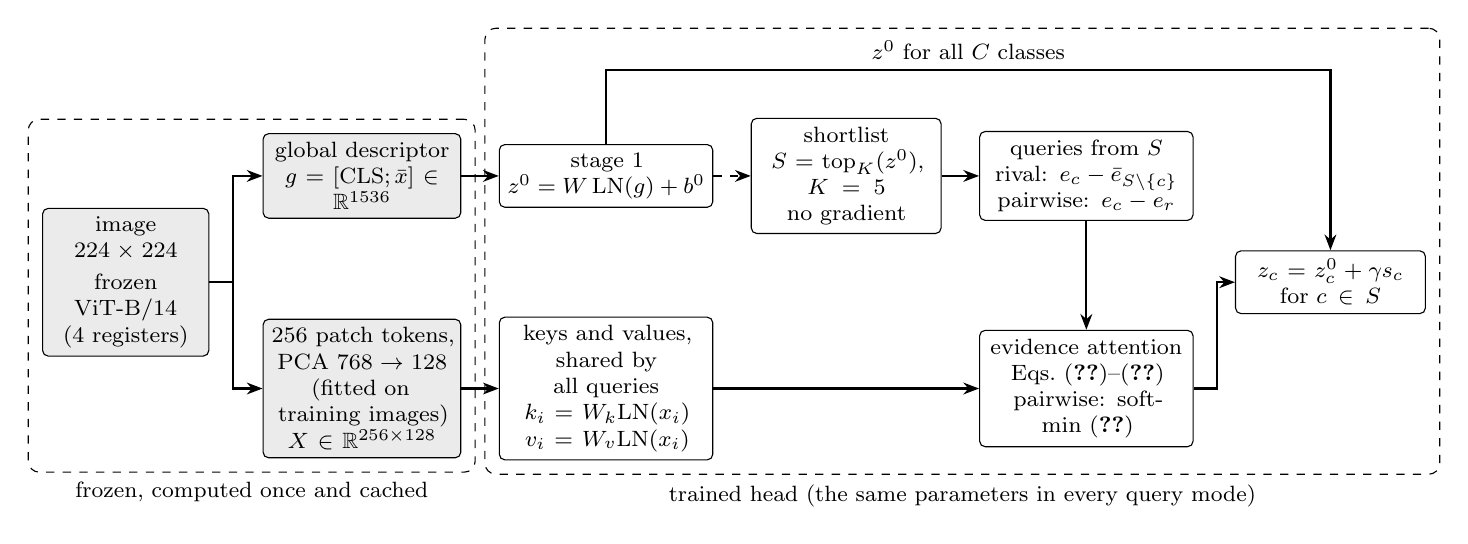
\begin{tikzpicture}[
  font=\footnotesize,
  box/.style={draw, rounded corners=2pt, align=center, inner sep=3pt},
  frozen/.style={box, fill=black!8},
  arr/.style={-{Stealth[length=2mm]}, thick},
  nograd/.style={arr, dashed},
  group/.style={draw, dashed, rounded corners=4pt, inner sep=5pt}]
\node[frozen, text width=1.9cm] (vit) at (0,0) {image\\$224\times224$\\[2pt]frozen ViT-B/14\\(4 registers)};
\node[frozen, text width=2.3cm] (g) at (3.0,1.35) {global descriptor\\$g=[\mathrm{CLS};\bar x]\in\R^{1536}$};
\node[frozen, text width=2.3cm] (X) at (3.0,-1.35) {256 patch tokens,\\PCA $768\to128$\\(fitted on training images)\\$X\in\R^{256\times128}$};
\node[box, text width=2.5cm] (z0) at (6.1,1.35) {stage 1\\$z^0=W\,\LN(g)+b^0$};
\node[box, text width=2.5cm] (kv) at (6.1,-1.35) {keys and values,\\shared by all queries\\$k_i=W_k\LN(x_i)$\\$v_i=W_v\LN(x_i)$};
\node[box, text width=2.2cm] (S) at (9.15,1.35) {shortlist\\$S=\topk(z^0)$, $K=5$\\no gradient};
\node[box, text width=2.5cm] (q) at (12.2,1.35) {queries from $S$\\rival: $e_c-\bar e_{S\setminus\{c\}}$\\pairwise: $e_c-e_r$};
\node[box, text width=2.5cm] (att) at (12.2,-1.35) {evidence attention\\Eqs.~(\ref{eq:attn})--(\ref{eq:score})\\pairwise: soft-min (\ref{eq:softmin})};
\node[box, text width=2.2cm] (out) at (15.3,0) {$z_c=z^0_c+\gamma s_c$\\for $c\in S$};
\coordinate (rt) at (6.1,3.05);
\node[group, fit=(vit)(g)(X)] (cache) {};
\node[anchor=north] at (cache.south) {frozen, computed once and cached};
\node[group, fit=(z0)(kv)(S)(q)(att)(out)(rt)] (head) {};
\node[anchor=north] at (head.south) {trained head (the same parameters in every query mode)};
\draw[arr] (vit.east) -- ++(0.3,0) |- (g.west);
\draw[arr] (vit.east) -- ++(0.3,0) |- (X.west);
\draw[arr] (g) -- (z0);
\draw[nograd] (z0) -- (S);
\draw[arr] (S) -- (q);
\draw[arr] (X) -- (kv);
\draw[arr] (kv) -- (att);
\draw[arr] (q) -- (att);
\draw[arr] (att.east) -- ++(0.3,0) |- (out.west);
\draw[arr] (z0.north) -- (6.1,2.7) -| node[pos=0.25, above] {$z^0$ for all $C$ classes} (out.north);
\end{tikzpicture}
\end{adjustbox}
\caption{RCEA. The frozen backbone runs once per image and its outputs are cached (grey). The trained head has a
linear stage 1 on $g$ and a second stage on the tokens: the shortlist is taken without gradient (dashed arrow), each
candidate's query is built from the shortlist, attends over the tokens and gives a score that is added to that
candidate's stage-1 logit; logits outside the shortlist pass through unchanged. The controls replace only the box
``queries from $S$''.}
\label{fig:pipeline}
\end{figure}

\begin{pseudocode}[!htbp]
\caption{One forward pass of the re-ranking head on a batch (as implemented in \texttt{CandidateReRanker.forward}).}
\label{alg:rcea}
\small
\begin{tabular}{@{}r@{\hspace{0.7em}}p{9.8cm}@{\hspace{0.8em}}>{\raggedright\arraybackslash\itshape}p{4.4cm}@{}}
 & \textbf{input:} $g\in\R^{B\times D_g}$, $X\in\R^{B\times N\times D}$, labels $y$ (training only) & \\
1 & $z^0\leftarrow W\,\LN(g)+b^0$ & stage-1 logits, $B\times C$\\
2 & $S\leftarrow\topk\bigl(\sg(z^0)\bigr)$ & indices, $B\times K$, no gradient\\
3 & \textbf{if} training \textbf{and} \fn{gt_insert}: for each image with $y\notin S$, put $y$ in the last slot of $S$ & the truth replaces the weakest candidate\\
4 & $E\leftarrow(e_c)_{c\in S}$ & $B\times K\times d$\\
5 & \textbf{if} mode is pairwise: $Q\leftarrow(e_c-e_r)_{c\in S,\,r\in S\setminus\{c\}}$ & $B\times K(K-1)\times d$\\
6 & \textbf{else}: $Q\leftarrow\mathrm{query}(E,\text{mode})$ & Eqs.~(\ref{eq:rival}), (\ref{eq:rivalsoft}) or a control (\ref{eq:controls})\\
7 & $k_i\leftarrow W_k\,\LN(x_i)$, $v_i\leftarrow W_v\,\LN(x_i)$, split into $H$ heads & once per image, shared by all queries\\
8 & $A\leftarrow\operatorname{softmax}_i\bigl((Q+b)^{\top}k_i/(\sqrt{d_h}\,\tau)\bigr)$ per head & training: each key masked with probability 0.1\\
9 & $R\leftarrow A\,V$ & $B\times H\times Q\times d_h$\\
10 & $s\leftarrow\sum_h\langle Q^{(h)},R^{(h)}\rangle/\sqrt{d_h}$ & one score per query\\
11 & \textbf{if} mode is pairwise: $s_c\leftarrow$ soft-min$_t$ of $(s_{c,r})_{r\neq c}$ & Eq.~(\ref{eq:softmin})\\
12 & $z\leftarrow z^0$; $z_c\leftarrow z_c+\gamma\,s_c$ for $c\in S$ & only the $K$ candidates move\\
13 & \textbf{return} $z$; in training the loss $\CE(z,y)+\alpha\,\CE(z^0,y)$ & Eq.~(\ref{eq:loss})\\
\end{tabular}
\end{pseudocode}

% =============================================================================================== 5 protocol
\section{Experimental protocol}\label{sec:protocol}

\subsection{Features}\label{sec:features}
The main backbone is DINOv2 ViT-B/14 with four registers (timm \fn{vit_base_patch14_reg4_}\allowbreak\fn{dinov2.lvd142m}), frozen,
at 224\,px. The evaluation transform resizes the shorter side to 256 pixels (bicubic), takes the centre
$224\times224$ crop and applies the ImageNet normalisation. The cache holds $g=[\mathrm{CLS};\bar x]$ (1536
dimensions) and the 256 patch tokens projected on a 256-component PCA. The PCA is fitted on the tokens of 4,000
randomly chosen training images (seed 0) of each dataset; Stanford Dogs has its own PCA. The 256 components keep
84.2\,\% of the token variance on Tsinghua Dogs and 83.3\,\% on Stanford Dogs. The heads read the first 128
components (32 or 64 in the token-width study). The first 32, 64 and 128 components keep 46.4, 58.8 and 71.7\,\% of
the token variance on Tsinghua Dogs, and 43.3, 56.3 and 70.0\,\% on Stanford Dogs (read from the saved PCA bases,
each fitted on 1,024,000 tokens).
The cached views are the original images of all three splits, the horizontally flipped training images, and the test
views of Section~\ref{sec:views}; for the transfer study the Stanford test images are also cached in the Tsinghua PCA
basis. Tokens are stored as float16. The backbone runs in fp16 autocast on the T4; the heads train and predict in
fp32. On Tsinghua Dogs the extraction ran at about 90--140 images per second, limited by the two CPU cores decoding
JPEGs, with a peak GPU memory of 1.20\,GB and a cache of 24\,GB. The training tokens (original and flipped, 7.7\,GB)
are kept on the GPU during training.

\subsection{Heads and training}\label{sec:training}
Nine heads are trained on each main dataset: the baselines B0, B1 and B2; the controls class, centre and random; and
the proposed rival, rival-soft and pairwise, all re-rankers with $K=5$ (Section~\ref{sec:method}). All heads use the
same optimiser, schedule, epochs and features (Appendix~\ref{app:hyper}): AdamW with weight decay 0.05 on weight
matrices and none on vectors; a linear warm-up over one epoch followed by cosine decay over at most 30 epochs; batch
size 256; gradient clipping at norm 1; label smoothing 0.1; token dropout with probability 0.1 for every head that
reads tokens (B1, B2 and all re-rankers); no dropout. Each training image uses its cached original or flipped view, chosen at random. Early stopping keeps the
epoch with the highest validation top-1 (ties: lower validation NLL) and stops after 8 epochs without a new best. The
test split is not loaded by any training script.

\subsection{Model selection, seeds and the freeze}\label{sec:selection}
For each head, the learning rate is chosen from $\{3\cdot10^{-4},10^{-3},3\cdot10^{-3}\}$ on seed 0 by validation
top-1 (ties: lower validation NLL). Seeds 0, 1 and 2 are then trained at that rate, so every head has three seed runs.
The ablation, open-set and token-width runs borrow the rate of the matching head of the Tsinghua main experiment and
select nothing themselves; each other backbone runs its own selection over the same grid, since one rate does not
carry over between feature spaces. In both main experiments every head chose $3\cdot10^{-4}$, the lowest rate in the grid (recorded in the
freezes of 20:13:39 and 21:03:42 UTC), and so did every head of the three other backbones. The best rate may lie below the grid; the grid was fixed before training and
was not widened afterwards, which is a limitation (Section~\ref{sec:limitations}).

The selection is frozen in code. \fn{scripts/freeze.py} writes, per experiment, the time, each head's rate and, for
every seed run, its validation metrics, best epoch and the SHA-256 of its checkpoint. Every evaluation script refuses
to run on an experiment without a freeze, on a run the freeze does not list, or on a checkpoint whose hash has
changed. The Stanford main experiment was frozen at 20:13:39 UTC and the Tsinghua main experiment at 21:03:42 UTC
on 8 November 2026, and both freeze summaries were entered in the research log before their test evaluations
(Appendix~\ref{app:freeze}). The seven secondary experiments are finished by a watcher (\fn{scripts/auto_final.sh},
declared in the log at 21:42 UTC, before any of them had finished), which freezes and then evaluates each one as soon
as its training ends. Their freeze summaries are copied into the log afterwards, from \fn{freeze.json}, whose time
stamp and the first time stamp of the evaluation log show the order. This departs from the stated order (freeze
recorded in the log before the evaluation); no choice is made between the end of training and the freeze.
Only one of the seven finished before the free-tier GPU runtime ended at about 22:14 UTC, after which Colab's
usage limit refused a new one: \fn{tsinghua_resnet50}, frozen at 21:56:00 UTC (12 runs, 4 heads) and evaluated
from 21:56:02 to 21:57:39 UTC, with its freeze summary entered in the log afterwards as described.
\fn{tsinghua_ablate} and \fn{tsinghua_convnext_tiny} were cut off during training, and \fn{tsinghua_openset},
\fn{tsinghua_clip_vitb16}, \fn{tsinghua_tok32} and \fn{tsinghua_tok64} never started. None of these six was frozen,
and no test split was read for any of them.

\paragraph{Resumption on Kaggle.} The six were finished on 9 November in a free-tier Kaggle session with two T4 GPUs
(\fn{scripts/kaggle_run.sh}), from the repository and the work folder mirrored on Google Drive (runs with their
checkpoints, logs, manifests and the saved token PCA basis), both packed as archives and checked by SHA-256 on arrival.
The feature caches had not been saved, so they were rebuilt from the three Tsinghua archives, downloaded again and
matched against the hashes of the Colab copies (Appendix~\ref{app:data}). The software differs (torch 2.11.0, cuDNN
92700, on Kaggle; torch 2.14.1, cuDNN 92800, on Colab), so the forward pass is not bit-identical. A resume rule,
recorded in the research log at 23:35 UTC on 8 November before any check had run, decided whether a cut-off
experiment keeps its finished runs: only if none of them, applied to the rebuilt validation features, moves its
validation top-1 by more than 0.001 (about 7 of 6,515 images); otherwise the whole experiment is trained again, so that
all its runs read the same features (\fn{scripts/feature_drift_check.py}, \fn{scripts/resume_policy.py}; no test split
is read). The frozen heads of \fn{tsinghua_main} were checked the same way, for the record. The largest change was
0.0003 for the 24 deterministic heads of \fn{tsinghua_main} (at most 3 of the 6,515 validation predictions changed) and
for the 22 finished ablation runs, and zero for the 6 finished ConvNeXt-T runs, so both experiments kept their
finished runs and trained only the missing ones. As declared, the random-rival control is not part of this
check, because its predictions depend on its random draws (59 to 82 of its validation predictions changed). A
watcher froze each experiment when its training ended and then evaluated it, as on Colab; both new backbones chose
the learning rate $3\cdot10^{-4}$ again for every head. The freezes (UTC) were \fn{tsinghua_convnext_tiny} at
02:40:25 (12 seed runs, 4 heads), \fn{tsinghua_ablate} at 03:06:03 (39 runs, 13 heads), \fn{tsinghua_clip_vitb16} at
03:08:16 (12, 4), \fn{tsinghua_openset} at 03:23:51 (12, 4), \fn{tsinghua_tok32} at 03:38:12 (9, 3) and
\fn{tsinghua_tok64} at 03:52:42 (9, 3). Each test evaluation began within a second of its freeze and took 18 to 69
seconds, and the freeze summaries were entered in the research log afterwards, as for \fn{tsinghua_resnet50}.

\subsection{Hypotheses and the decision rule}\label{sec:rule}
The hypotheses (Table~\ref{tab:hyp-design}) and the decision rule were written down before the first training run
and made mechanical by seven analysis rules recorded before any test evaluation (Appendix~\ref{app:rules}). The primary
metric is test top-1, and Tsinghua Dogs is the primary dataset. For a comparison of head A with head B on seed $s$,
let $\Delta_s$ be the difference of their test top-1 on the same test images and $[\ell_s,u_s]$ its paired bootstrap
95\,\% interval. The rule reads
\begin{equation}
\text{``$A>B$''}\iff\Delta_s>0\ \text{for all } s\in\{0,1,2\}\ \text{and}\ \ell_s>0\ \text{for at least two } s,
\label{eq:rule}
\end{equation}
symmetrically for ``$B>A$'' (all $\Delta_s<0$ and $u_s<0$ for at least two seeds); otherwise no claim is made, and a
comparison with fewer than three seeds is incomplete. The exact McNemar test is reported beside it but is not part of
the rule. The rule is applied to the numbers as they come out, and a refuted hypothesis is reported as refuted.

\begin{table}[!htbp]
\centering
\caption{The seven hypotheses as fixed before training (design document, Sec.~8); names shortened, predictions
and refutation criteria as there. ``The rule'' is Eq.~\eqref{eq:rule}.}
\label{tab:hyp-design}
\small
\begin{tabularx}{\textwidth}{@{}lL{3.1cm}YL{4.3cm}@{}}
\toprule
 & Hypothesis & Prediction & Refuted if\\
\midrule
H1 & Shortlist conditioning matters & rival, rival-soft or pairwise $>$ class, centre and random on the Tsinghua test
split; the same sign on the Stanford test split & the best proposed mode does not exceed the best control by the
rule\\
H2 & It acts where it should & among images whose truth is in $S$ but not top-1 under $z^0$, fixes far outnumber
breaks; the gain over B0 concentrates in the 20 breed pairs most confused by B0 & fix rate $\le$ break rate, or the
gain on the 20 pairs is no larger than the overall gain\\
H3 & It is the confusion set, not contrast in general & random $\le$ centre & random within the seed spread of
rival\\
H4 & Pairwise evidence adds beyond centring & pairwise $\ge$ rival at $K=5$ (identical at $K=2$, Fact~\ref{fact:pairwise}) &
exploratory; reported either way\\
H5 & The shortlist costs nothing & re-ranking $\ge$ B2 at $1/26$ of its per-query cost & B2 is ahead by the rule\\
H6 & $K$ behaves like a shortlist & over $K\in\{2,3,5,10\}$ the shortlist recall rises with $K$ and accuracy is flat or
peaks at a small $K$ & accuracy falls monotonically from $K=2$\\
H7 & Robustness (exploratory) & under corruptions that lower top-1 but keep the top-$K$ recall, the re-ranker
recovers more than B0 & reported either way\\
\bottomrule
\end{tabularx}
\end{table}

\paragraph{How the hypotheses are evaluated.} The table code computes every verdict from the digest.
\emph{H1}: the best proposed mode and the best control are the tags with the highest mean validation top-1 over their
three seed runs on Tsinghua Dogs (ties: lower mean validation NLL); Stanford Dogs repeats the same pair, and its own
validation picks are reported beside it. H1 is supported if the pair gives ``$A>B$'' on Tsinghua and a positive mean
difference on Stanford. Applied to the frozen validation predictions of the Tsinghua main experiment, this rule names
rival-soft as the best proposed mode and the class query as the best control; H2, H5 and H7 use rival-soft.
\emph{H2}: a fix is an image whose stage-1 top-1 is wrong and whose final top-1 is right, a break the reverse. The
code compares the two rates over all test images, which compares their numbers; the design's restriction to images
with the truth in $S$ changes nothing for breaks, and for fixes only the rare case in which all $K$ candidates are
pushed below a truth outside $S$. The hard pairs are the 20 unordered breed pairs with most confusions in either direction in the validation
predictions of B0, seed 0.
\emph{H3}: ``within the seed spread'' means $|\text{random}-\text{rival}|$ is at most the larger of their two test
top-1 standard deviations over seeds; if not, H3 is supported when random $\le$ centre and partly supported otherwise.
\emph{H5}: refuted if B2 is ahead by the rule; supported with ``re-ranker ahead'' or ``no difference'' otherwise.
\emph{H6}: uses the rival head; refuted if top-1 falls strictly from $K=2$ to 3, 5 and 10. \emph{H4} and \emph{H7} are
exploratory and reported as the rule's outcome and as the per-view gains over B0 against the clean gain.

\subsection{Comparisons}\label{sec:comparisons}
The pairs are fixed in \fn{scripts/final_all.sh} together with the views and their order.
On the clean test view of both main experiments there are 22 pairs: each proposed head against each of the three
controls (9 pairs); pairwise and rival-soft against rival; the control chain random against centre and centre against
class; each proposed head against B2 (3); each proposed head and the class query against B0 (4); rival and pairwise
against B1. Table~\ref{tab:isolates} lists what the main comparisons isolate. On every corrupted or
annotation-assisted view, 7 pairs are compared: rival, rival-soft, pairwise and class against B0, and rival,
rival-soft and pairwise against class. The ablation compares rival with class at $K=2,3,10$ and pairwise with rival at
$K=3,10$; each other backbone compares rival and pairwise with class, pairwise with rival, and rival and class with
B0; the token-width runs compare rival with class and rival and class with B1. The provenance subsets repeat the 22
clean-view pairs (Section~\ref{sec:protocol-provenance}).

\begin{table}[!htbp]
\centering
\caption{What each main comparison isolates. All pairs are evaluated on the clean test view of both main
experiments.}
\label{tab:isolates}
\small
\begin{tabularx}{\textwidth}{@{}L{4.6cm}Y@{}}
\toprule
Comparison & Isolates\\
\midrule
class (re-ranking) vs B0 & a second look at the patches with class-specific queries (CSRA on the shortlist)\\
centre vs class & centring alone (global, the same for every image)\\
random vs centre & contrast against a random set of classes\\
rival vs random & contrast against the image's own confusion set (the claim)\\
rival-soft vs rival & weighting the rivals by the stage-1 belief\\
pairwise vs rival & pairwise evidence against shortlist centring ($K\ge3$)\\
re-ranking vs B2 & shortlist against all classes, at equal parameters\\
re-ranking vs B1 & class-conditional against class-agnostic attention, at similar capacity\\
\bottomrule
\end{tabularx}
\end{table}

\subsection{Statistics}\label{sec:stats}
Every head has three seed runs. Summaries are the mean and standard deviation over seeds (with $n-1$ in the
denominator) and a $t$-based 95\,\% interval. Paired comparisons are made seed by seed on the same test images: a
percentile bootstrap of the top-1 difference with 10,000 resamples of the test images (generator seed 0), and the
exact McNemar test on the discordant images (a two-sided binomial test of $n_{10}$ out of $n_{10}+n_{01}$ with
probability $1/2$). The verdict is Eq.~\eqref{eq:rule}. For the random control, the standard deviation of its test
top-1 over five further draws of the random classes (generator seeds $s,1000+s,\dots,4000+s$ for seed run $s$) is
reported as \fn{top1_draw_sd}. Appendix~\ref{app:stats} gives the details.

\subsection{Metrics}\label{sec:metrics}
Top-1 and top-5 accuracy; macro precision, recall and F1; NLL, expected calibration error (15 equal-width bins) and
Brier score, raw and after temperature scaling, with the temperature fitted on the run's validation
predictions~\citep{guo2017calibration,naeini2015bbq}; the area under the risk--coverage curve and the risk at 90\,\%
coverage of the maximum softmax probability~\citep{geifman2017selective}. For re-ranking heads also: the stage-1
top-1, the shortlist recall (truth in $S$), and the shares of all test images whose top-1 the second stage changes,
fixes (stage 1 wrong, final right) or breaks (stage 1 right, final wrong). Per breed: the test accuracy of each head.
For the hard pairs: the test errors within the 20 pairs and the accuracy on the test images of their breeds.

\subsection{Test views}\label{sec:views}
Each view is applied to the full image before the evaluation transform, deterministically, with the image id as seed
(Table~\ref{tab:views}). The automatic views use no annotation. The annotation-assisted views use the dataset's
ground-truth boxes at test time. They are robustness probes and are never reported as automatic inference; their
results are kept in a separate block of every table and figure. Stanford Dogs has body boxes only, so it has three
annotation-assisted views. H7 uses the automatic views only.

\begin{table}[!htbp]
\centering
\caption{Test views. Grey is (124, 116, 104), the ImageNet mean. An annotation-assisted view leaves an image unchanged
when the image has no usable box.}
\label{tab:views}
\small
\begin{tabularx}{\textwidth}{@{}lYll@{}}
\toprule
View & What it does & Boxes at test time & Datasets\\
\midrule
clean & none (the evaluation transform only) & no & both\\
blur & Gaussian blur, radius 3 & no & both\\
noise & additive Gaussian noise, $\sigma=25$ on the 0--255 scale & no & both\\
JPEG & re-encoding at JPEG quality 10 & no & both\\
low resolution & bilinear down-sampling by 4 and back up & no & both\\
occlusion & a grey square covering 25\,\% of the image at a seeded position & no & both\\
\midrule
head occlusion & the head box painted grey & yes & Tsinghua\\
grey background & everything outside the body box painted grey & yes & both\\
blurred background & everything outside the body box blurred, radius 12 & yes & both\\
body crop & crop to the body box with a 10\,\% margin & yes & both\\
head crop & crop to the head box with a 10\,\% margin & yes & Tsinghua\\
\bottomrule
\end{tabularx}
\end{table}

\subsection{Open set with held-out breeds}\label{sec:protocol-openset}
30 of the 130 Tsinghua breeds are drawn at random (seed 0) and held out; the draw is stored in
\fn{configs/openset/tsinghua_unknown30_s0.json}. B0 and the class, rival and pairwise re-rankers are trained on the
remaining 100 breeds, with no image of a held-out breed in training or validation, at the rates of the main
experiment. On the test split, the images of the 100 known breeds are in-distribution and those of the 30 held-out
breeds are unknown. Scores (larger means known): maximum softmax probability, raw and temperature-scaled; maximum
logit; energy (log-sum-exp of the logits); and the top-1 minus top-2 logit margin; for re-rankers also the same scores
of the stage-1 logits. Metrics: AUROC and the false-positive rate at 95\,\% true-positive rate (threshold at the
5\,\% quantile of the known images' scores), and closed-set top-1 on the known breeds. Two caveats hold by
construction: the held-out breeds are unknown to the heads but not to the backbone, and the token PCA is the main
one, fitted without labels on training images of all 130 breeds.

\subsection{Transfer to de-duplicated Stanford Dogs}\label{sec:protocol-transfer}
Heads trained on Tsinghua Dogs label Stanford Dogs test images without any training on Stanford Dogs. The breed
correspondence is the one the audit measured: for each Tsinghua breed, the majority Stanford breed among its
confirmed pairs. A Stanford breed is used only if exactly one Tsinghua breed maps to it, with a purity of at least 0.9
and at least 5 pairs. The images are the 973 clean Stanford test images (no candidate in the Tsinghua training or
validation data) of the mapped breeds, with tokens in the Tsinghua PCA basis. The prediction is the full 130-breed
Tsinghua decision and counts as correct when it is the mapped breed; a second number restricts the decision to the
mapped breeds. These images are still ILSVRC-2012 training images (Section~\ref{sec:pretrain-overlap}).

\subsection{Provenance subsets}\label{sec:protocol-provenance}
\fn{scripts/subset_eval.py} re-scores the saved test predictions of the Tsinghua main experiment on the subsets of
Section~\ref{sec:provenance} (all, Stanford-origin, independent) and repeats the 22 clean-view comparisons on each.
Nothing is trained or selected on the subsets, and they were fixed by the audit before any test prediction existed.

\subsection{Other backbones}\label{sec:protocol-backbones}
Three further frozen backbones are run on Tsinghua Dogs with B0 and the class, rival and pairwise re-rankers: CLIP
ViT-B/16 (timm \fn{vit_base_patch16_clip_224.openai}, WIT-400M; 196 tokens; $g=[\mathrm{CLS};\bar x]$ of 1536
dimensions; CLIP's own normalisation), ResNet-50 (torchvision \texttt{IMAGENET1K\_V2}; 49 tokens of 2048 dimensions;
$g$ the average-pooled feature) and ConvNeXt-T (torchvision \texttt{IMAGENET1K\_V1}; 49 tokens of 768 dimensions; $g$ the
average). Each has its own 256-component token PCA (first 128 components used), its own learning-rate grid, and only
the clean and flipped views; it is evaluated on the clean test view only.

\subsection{Efficiency}\label{sec:protocol-efficiency}
\fn{scripts/efficiency_report.py} measures, on the runtime's device (whose name it records) and with nothing else on
the GPU: parameters; FLOPs from \texttt{torch.utils.flop\_counter}, where a multiply-add counts as 2 FLOPs; median
latency over 50 timed passes after 10 warm-up passes; and peak GPU memory. It covers every head on random inputs of
the cached shapes at batch 1 and 256 (fp32), the frozen backbone at batch 1 and 64 (fp16 autocast), and the full
single-image pipeline (backbone, token PCA, head). It reads no test data and is not part of the locked evaluation.

\subsection{Attention against the boxes}\label{sec:protocol-explain}
\fn{scripts/explain.py} records, for seed 0 of each head on the Tsinghua test split, the attention over the token grid,
averaged over attention heads (for pairwise, also over the candidate's rival pairs): for re-rankers the map of the
final top-1 candidate, for B1 the mean of its queries, for B2 the map of the predicted class. Using the dataset's
head and body boxes for this measurement only, it reports the attention mass inside each box, the box's share of the
image (what a uniform map would give), their ratio (the lift; above 1 means the map prefers the box) and the entropy
of the map relative to a uniform one. Its figure is chosen without hand-picking: the first images by id of each kind
(the rival head fixed a stage-1 error, broke a correct stage-1 answer, or both were right), with the maps of the two
highest-scoring final candidates of the rival and class heads.

% =============================================================================================== 6 results
\section{Results}\label{sec:results}

Each table and figure is produced from the result digest (\fn{results/digest}, 15 files whose SHA-256 are listed in
its \fn{MANIFEST.txt}) by \fn{scripts/make_tables.py} and \fn{scripts/make_figures.py}. The secondary studies were
finished on Kaggle and merged into the digest with \fn{scripts/ingest_kaggle.sh}, which checks the result archives
against their SHA-256 and requires the archive's run registry to contain every row of the earlier one. The numbers in
the text are read from the same tables and from \fn{paper/generated/numbers.json}. Differences are in percentage points (pp) of test
top-1 unless stated otherwise, and ``mean'' is the mean over the three seed runs.

\subsection{Main results}\label{sec:res-main}
On Tsinghua Dogs the three baselines are level: 86.26\,\% (B0), 86.26\,\% (B1) and 86.28\,\% (B2) test top-1
(Table~\ref{tab:main-tsinghua}). Every re-ranking head is above them, from 86.43\,\% for random rivals to
87.12\,\% for rival-soft, the highest mean (standard deviation 0.15 over seeds); top-5 lies between 98.45 and
98.58\,\% for all nine heads, and macro-F1 follows top-1 (86.23\,\% for B0, 87.00\,\% for rival-soft). On Stanford
Dogs the picture differs (Table~\ref{tab:main-stanford}): B0 (88.33\,\%), B2 (88.34\,\%) and the six re-rankers
(88.16--88.28\,\%) lie within 0.2 points of each other, and the attentive probe trails at 86.71\,\%. Which of these
differences the rule supports is stated in Section~\ref{sec:res-hyp} and Table~\ref{tab:compare}.

After temperature scaling every head is well calibrated, with ECE between 1.16 and 1.61\,\% on Tsinghua Dogs and
between 1.16 and 1.49\,\% on Stanford Dogs. On Tsinghua Dogs the re-rankers have a lower NLL (0.461--0.472 against
0.479--0.482 for the baselines) and Brier score (0.217--0.225 against 0.231--0.233), rival-soft the lowest of both,
and selective prediction follows: the area under the risk--coverage curve (AURC) is 3.36\,\% for rival-soft against
3.74\,\% for B0, and the error rate on the 90\,\% most confident test images is 8.74\,\% against 9.46\,\%. On
Stanford Dogs B0 has the lowest NLL (0.402; the others 0.406--0.413, B1 0.453), and the AURC is 2.76--2.85\,\% for
every head except B1 (3.53\,\%). No test was pre-registered for these metrics; they are descriptive.

\gentable{main_tsinghua}{Tsinghua Dogs test split (5,200 images): the nine heads on the same frozen DINOv2 features.
Mean and standard deviation over three seeds of top-1, top-5, macro precision, recall and F1, and of NLL and ECE
after temperature scaling fitted on validation. Bold marks the highest mean top-1; differences between heads are
judged only by the paired comparisons of Table~\ref{tab:compare}.}{tab:main-tsinghua}

\gentable{main_stanford}{Stanford Dogs test split (8,580 images), read as Table~\ref{tab:main-tsinghua}. Absolute
values are optimistic for every head, since every Stanford Dogs image is an ILSVRC-2012 training image
(Section~\ref{sec:pretrain-overlap}).}{tab:main-stanford}

\genfigure{main}{Test top-1 of every head, mean and $t$-based 95\,\% interval over three seeds, one panel per
dataset; the colour gives the family (baselines, controls, proposed). The intervals describe seed-to-seed spread;
differences between heads are judged by the paired tests of Figure~\ref{fig:compare}, not by whether these intervals
overlap.}{fig:main}

\subsection{The hypotheses under the decision rule}\label{sec:res-hyp}
Table~\ref{tab:hypotheses} gives the verdicts as computed. Each paragraph below states the verdict first and then the
evidence; a refuted hypothesis is reported as refuted.

\gentable{hypotheses}{H1--H7 as judged by the pre-registered rule (Eq.~\eqref{eq:rule} and
Section~\ref{sec:rule}): verdict and evidence, computed by \texttt{make\_tables.py} from the digest. Tsinghua Dogs is
primary; Stanford Dogs gives the sign check of H1. The table's ``\S8'' is Section~8 of the design document, i.e.\ the
rule of Eq.~\eqref{eq:rule}.}{tab:hypotheses}

\paragraph{H1, shortlist conditioning: refuted.}
Validation names rival-soft as the best proposed mode and the class query as the best control. On the Tsinghua test
split rival-soft is ahead in every seed, by $+0.37$, $+0.50$ and $+0.37$ points, but only the second seed's paired
interval excludes zero ($[+0.10,+0.90]$; the other two are $[-0.12,+0.85]$ and $[-0.10,+0.83]$), so the rule makes no
claim; the largest exact McNemar $p$ over the seeds is 0.17. On Stanford Dogs the same pair differs by $+0.05$,
$+0.15$ and $-0.28$ points (no claim), and Stanford's own validation picks, pairwise and random rivals, give no claim
either. The verdict does not change on the provenance subsets: $+0.37$ points on the Stanford-origin images and
$+0.69$ on the independent ones, both without a claim (Section~\ref{sec:res-provenance}).

\paragraph{H2, where it acts: supported on Tsinghua Dogs, refuted on Stanford Dogs.}
Rival-soft's second stage fixes 1.91\,\% of the Tsinghua test images (wrong at stage 1, right after re-ranking) and
breaks 0.68\,\%. On the test images of the breeds in the 20 hard pairs its gain over B0 is $+1.34$ points, against
$+0.86$ overall. This concentration is not specific to rival conditioning: the class query ($+0.69$ against $+0.45$),
the pairwise head ($+1.56$ against $+0.53$) and the attentive probe ($+0.94$ against $0.00$) show it too
(Table~\ref{tab:hardpairs-tsinghua}). On Stanford Dogs fixes and breaks are equal (0.42\,\% each), and the gain on its
own 20 pairs is $-0.12$ points against $-0.08$ overall.

\paragraph{H3, confusion set or contrast: supported by its criterion; the paired rule makes no claim.}
Random rivals reach 86.43\,\%, centring 86.49\,\% and rival 86.74\,\%. Random lies outside the seed spread of rival
($|86.43-86.74|=0.31$ points against a larger standard deviation of 0.23) and does not exceed centring, so H3 is
supported as defined in Section~\ref{sec:rule}. The paired comparison is weaker: rival minus random is $+0.31$ points
with one of three intervals excluding zero, so the rule itself makes no claim for rival over random; it does for
rival-soft over random ($+0.69$). The random control's standard deviation over five further draws of its random
classes is 0.07 points on Tsinghua Dogs and 0.04 on Stanford Dogs (\fn{top1_draw_sd}), well below the spread over
seeds. On Stanford Dogs random (88.16\,\%) lies within the spread of rival (88.17\,\%), and H3 is refuted there.

\paragraph{H4, pairwise evidence: no difference (exploratory).}
Pairwise minus rival at $K=5$ is $+0.06$ points on Tsinghua Dogs (per seed $+0.13$, $-0.12$, $+0.15$; no claim) and
$+0.01$ on Stanford Dogs (no claim). On Stanford Dogs the two heads make almost the same decisions: the per-seed
differences are $+0.00$, $+0.01$ and $+0.01$ points. On Tsinghua Dogs the ablation repeats the pair at other
shortlist sizes: pairwise minus rival is $+0.15$ points at $K=3$ (per seed $+0.15$, $+0.13$, $+0.17$) and $+0.15$ at
$K=10$ ($+0.37$, $+0.00$, $+0.10$). At $K=3$ every seed is positive, but no paired interval excludes zero and the
smallest McNemar $p$ is 0.45, so the rule makes no claim at either size.

\paragraph{H5, cost of the shortlist: supported, with the re-ranker ahead on Tsinghua Dogs.}
Rival-soft beats class attention over all classes (B2) by $+0.84$ points, with every seed's interval above zero
($+0.92$, $+0.65$, $+0.94$; largest McNemar $p$ 0.0024). On Stanford Dogs the difference is $-0.09$ points with no
claim, which the hypothesis also counts as support (no difference). The measured cost agrees with the count of
Section~\ref{sec:complexity} (Table~\ref{tab:efficiency}): rival-soft needs 35.3 MFLOPs per image against B2's 68.0,
about half, since only the queries' share, $1/26$ of B2's, shrinks with $K$, while both heads compute the keys and
values of the 256 tokens once per image. On the T4, a batch of 256 images takes rival-soft 6.5\,ms and B2 14.7\,ms,
with peak memory 625 against 929\,MB. For a single image B2 is the faster head (0.53 against 0.86\,ms); the full
single-image pipeline takes 8.6\,ms with rival-soft and 8.7\,ms with B2, against 8.4\,ms for the backbone alone.

\paragraph{H6, shortlist size: supported by its criterion, within the seed spread.}
The rival head reaches 86.85\,\% test top-1 at $K=2$, 86.91\,\% at $K=3$, 86.74\,\% at $K=5$ and 86.52\,\% at
$K=10$, while its shortlist recall rises from 94.19 through 96.77 and 98.47 to 99.37\,\% (Table~\ref{tab:ablate-k},
Figure~\ref{fig:ksweep}). Top-1 does not fall strictly from $K=2$, so H6 is supported as defined in
Section~\ref{sec:rule}: accuracy is flat or peaks at a small $K$. The support is weak. The rise from $K=2$ to $K=3$
is $+0.06$ points and the fall from $K=3$ to $K=10$ is $0.39$ points, against seed standard deviations of 0.05 to
0.23. The pre-registered pairs compare heads at the same $K$ only, so the rule makes no claim across sizes. The $K=5$
values come from the main experiment, evaluated on the Colab feature cache; the other sizes were trained and evaluated
on the rebuilt cache (Section~\ref{sec:selection}). The other two heads of the study show how fragile the support
is: the class query falls strictly from $K=2$ (86.83, 86.73, 86.71 and 86.42\,\%), which would refute H6 had it been
stated for that head, and the pairwise head falls from $K=3$ (87.06, 86.80 and 86.67\,\%).

\paragraph{H7, robustness: exploratory.}
On Tsinghua Dogs rival-soft's gain over B0 is $+0.86$ points on the clean view and $+3.03$ (blur), $+0.83$ (noise),
$+0.76$ (JPEG), $+1.73$ (low resolution) and $+2.64$ points (occlusion) on the automatic corruptions; the rule gives
``rival-soft $>$ B0'' on all five. The gain exceeds the clean gain under occlusion, blur and low resolution, the
three views where the rival head's shortlist recall falls most (89.5, 93.9 and 96.7\,\%, against 98.5\,\% clean),
and not under JPEG and noise, where it falls least (96.9 and 97.7\,\%). The pattern therefore does not follow the
condition the prediction named, corruptions that keep the recall. On Stanford Dogs the gain lies between $-0.07$ and
$-0.23$ points on every automatic view, with no claim.

\subsection{Controls and the query axis}\label{sec:res-controls}
Along the query axis no step reaches a claim on Tsinghua Dogs (Table~\ref{tab:compare}): centre minus class is
$-0.22$ points, random minus centre $-0.06$ and rival minus random $+0.31$; rival-soft minus rival is $+0.38$, also
without a claim. Of the nine pairs of a proposed head against a control, two reach ``$A>B$'', both for rival-soft:
over centring ($+0.63$) and over random rivals ($+0.69$, largest McNemar $p$ 0.015). Neither rival nor pairwise beats
any control. Against the baselines the rule is more favourable: each proposed head beats B2 (rival $+0.46$, rival-soft
$+0.84$, pairwise $+0.51$) and B0 ($+0.47$, $+0.86$, $+0.53$), and pairwise beats B1 ($+0.53$), whereas the class
query, a control with the same parameters, does not beat B0 ($+0.45$, no claim). On Stanford Dogs the only claims are
rival and pairwise over the attentive probe ($+1.46$ and $+1.47$); every other pair gives no claim.

The second stage changes few decisions (Table~\ref{tab:rerank}). On Tsinghua Dogs the stage-1 heads of the
re-rankers reach 85.89--86.19\,\% top-1, slightly below B0, and their shortlists hold the true breed for
98.40--98.54\,\% of the test images at $K=5$. Re-ranking adds $+0.37$ (centred query) to $+1.23$ points
(rival-soft). Rival-soft changes the decision for 3.56\,\% of the test images: it fixes 1.91\,\%, breaks 0.68\,\%, and
in the remaining 0.97\,\% replaces one wrong breed by another. On Stanford Dogs the stage-1 heads already reach
88.19--88.36\,\%, re-ranking moves top-1 by $-0.08$ to $+0.00$ points, and among the changed decisions
(0.49--1.10\,\% of the images) breaks are as frequent as fixes or slightly more frequent (fixes 0.16--0.42\,\%, breaks
0.21--0.42\,\%).

\gentable{compare}{Paired comparisons on the clean test view: the 22 pairs fixed in \texttt{final\_all.sh}, per
dataset. For each pair A $-$ B: the mean difference in test top-1 over seeds (percentage points), the difference of
each seed with its paired bootstrap 95\,\% interval, the largest exact McNemar $p$-value over the seeds, and the
verdict of the rule; ``no claim'' means that the rule's condition holds in neither direction. The dagger marks the
H1 pair.}{tab:compare}

\genfigure{compare}{Forest plot of the paired comparisons on the clean test view: for each pair A $-$ B and each seed,
the difference in test top-1 (percentage points) with its paired bootstrap 95\,\% interval; the rule's verdict is
printed on the right. A pair reaches ``A $>$ B'' only when all three points lie right of zero and at least two
intervals exclude zero.}{fig:compare}

\gentable{rerank}{What the second stage does, per re-ranking head and dataset: the top-1 of the head's own stage 1,
the final top-1, their difference, the shortlist recall at $K=5$, and the shares of test images whose top-1 the
second stage changes, fixes (wrong to right) and breaks (right to wrong). All in \% of the test images; mean and
standard deviation over seeds.}{tab:rerank}

\subsection{Ablations: shortlist size, training choices and token width}\label{sec:res-ablation}
All three studies use Tsinghua Dogs and the learning rates of the main experiment. 22 of the ablation's 39 runs were
trained on Colab and kept by the resume rule; its other 17 runs and all token-width runs were trained on Kaggle
(Section~\ref{sec:selection}). The studies use rival, not the H1-selected rival-soft, as the proposed head
(Section~\ref{sec:limitations}).

\paragraph{Shortlist size.} Raising $K$ from 2 to 10 lifts the rival head's shortlist recall from 94.19 to
99.37\,\% but not its top-1, which stays between 86.52 and 86.91\,\% (Table~\ref{tab:ablate-k},
Figure~\ref{fig:ksweep}; H6). At every size the class query and rival lie within 0.2 points of each other: rival minus
class is $+0.03$ points at $K=2$, $+0.18$ at $K=3$ and $+0.10$ at $K=10$, with no claim at any size (and $+0.03$ at
$K=5$). Of the three heads, pairwise is the most accurate at $K=3$ (87.06\,\%), $+0.15$ points above rival without a
claim (H4).

\paragraph{Training choices.} No single change moves test top-1 by more than 0.15 points from the main head of its
mode (Table~\ref{tab:ablate-other}). Computing the loss over the shortlist only costs rival 0.14 points; dropping the
insertion of the true class into the training shortlist, or the token dropout, changes it by $+0.08$ and $+0.02$
points; replacing the soft minimum over pairs by a hard one ($t\to0$) or a softer one ($t=3$) changes pairwise by
$-0.15$ and $-0.03$ points. These differences are smaller than the seed standard deviations of several variants (up
to 0.35 points). The pre-registered pairs do not compare a variant with the main head, which belongs to another
experiment, so the differences are descriptive; none of the three training choices of the main configuration is
shown to matter.

\paragraph{Token width.} Keeping 32 or 64 instead of 128 principal components of the patch tokens costs each head 0.1
to 0.4 points (Table~\ref{tab:tokens}): rival reaches 86.58 and 86.63\,\% against 86.74\,\%, the class query 86.49 and
86.56 against 86.71\,\%, and B1 86.07 and 85.90 against 86.26\,\%. At both narrower widths the rule finds the class
query and rival ahead of B1 ($+0.42$ and $+0.51$ points at 32 dimensions, $+0.66$ and $+0.74$ at 64), which it does not
find for rival at 128 dimensions ($+0.47$, no claim). Rival minus class is $+0.08$ points at both widths, with no
claim.

\gentable{ablate_k}{Shortlist size $K$ on Tsinghua Dogs: test top-1 (\%) of the class, rival and pairwise heads at
$K=2,3,5,10$ ($K=5$ from the main experiment), and the test shortlist recall of the rival head. At $K=2$ pairwise
equals rival (Fact~\ref{fact:pairwise}) and was not trained separately.}{tab:ablate-k}

\genfigure[0.75\textwidth]{ksweep}{Test top-1 (left) and test shortlist recall (right) of the rival head against the
shortlist size $K$ on Tsinghua Dogs (logarithmic axis), mean and 95\,\% interval over seeds.}{fig:ksweep}

\gentable{ablate_other}{One change at a time from the main configuration on Tsinghua Dogs: validation and test top-1
(\%) of each variant and its test difference to the main head of the same mode, at the learning rate of that main
head.}{tab:ablate-other}

\gentable{tokens}{Token width on Tsinghua Dogs: test top-1 (\%) of B1 and of the class and rival re-rankers when the
patch tokens keep 32, 64 or 128 principal components (learning rates of the main experiment).}{tab:tokens}

\subsection{Robustness}\label{sec:res-robust}
The two kinds of view are reported apart. Automatic views use no annotation and measure robustness of automatic
inference; annotation-assisted views use the ground-truth boxes at test time and are probes only.
\paragraph{Automatic views.} Every head loses accuracy under every corruption on Tsinghua Dogs, most under
occlusion (B0 67.7\,\%, rival-soft 70.3\,\%) and blur (74.2 and 77.3\,\%) and least under noise (83.9 and
84.7\,\%; Table~\ref{tab:robust-tsinghua}). Rival-soft is the most accurate head on every automatic view. Of the 7
comparisons per view, the rule gives ``rival-soft $>$ B0'' and ``rival $>$ B0'' on all five corruptions, and
``rival-soft $>$ class'' under blur, low resolution and occlusion ($+1.87$, $+0.88$, $+2.05$ points) but not under
noise or JPEG ($+0.28$, $+0.03$). The rival head beats the class query only under blur ($+0.85$), as does the
pairwise head ($+0.78$); the class query itself beats B0 under blur, noise, JPEG and low resolution but not under
occlusion. The rival head's shortlist recall at $K=5$ falls from 98.5\,\% (clean) to 97.7 (noise), 96.9 (JPEG),
96.7 (low resolution), 93.9 (blur) and 89.5\,\% (occlusion). On Stanford Dogs the heads other than B1 lie within 0.8
points of each other on every automatic view, and none of the 7 comparisons reaches a claim on any view
(Table~\ref{tab:robust-stanford}).

\paragraph{Annotation-assisted views (ground-truth boxes at test time; probes, not automatic inference).} On Tsinghua
Dogs, covering the head box costs every head most: B0 falls to 46.8\,\% and rival-soft to 51.1\,\%, and the rival
head's shortlist recall to 74.1\,\%. Rival-soft keeps its largest lead there, $+4.33$ points over B0 and $+3.51$ over
the class query, both ``$A>B$''. Greying the background costs B0 0.6 points and blurring it 1.7; cropping to the body
box leaves B0 at 86.3\,\%, and cropping to the head box gives 84.4\,\%. Rival-soft is ahead of B0 by the rule on the
grey and blurred backgrounds and the body crop ($+0.79$, $+0.72$, $+0.73$) and ahead of the class query on the two
background views ($+0.69$, $+0.72$); none of the 7 comparisons reaches a claim on the head crop. On Stanford Dogs,
which has body boxes only, no comparison reaches a claim on these views either.

\gentable{robust_tsinghua}{Tsinghua test top-1 (\%) per view, mean over seeds. Left block: automatic views (clean and
five corruptions; no annotation used). Right block: annotation-assisted views, which use the dataset's ground-truth
boxes at test time and are robustness probes, not automatic inference. Last row: shortlist recall at $K=5$ of the
rival head.}{tab:robust-tsinghua}

\gentable{robust_stanford}{Stanford test top-1 (\%) per view, read as Table~\ref{tab:robust-tsinghua}; Stanford Dogs
has body boxes only, so its annotation-assisted views are the grey background, the blurred background and the body
crop.}{tab:robust-stanford}

\genfigure{robust}{Gain in test top-1 over B0 (percentage points) under each view, for the H1-selected proposed head,
the H1-selected control, the class query if different, and B2. Automatic views form the upper group of rows;
annotation-assisted views, which use ground-truth boxes at test time, form the lower group.}{fig:robust}

\subsection{Open set}\label{sec:res-openset}
The draw holds out 30 breeds: Shiba dog, French bulldog, Pomeranian, cairn, Australian terrier, Pembroke, Bedlington
terrier, Sussex spaniel, bluetick, standard schnauzer, wire-haired fox terrier, whippet, kuvasz, groenendael, malinois,
Great Pyrenees, English foxhound, Eskimo dog, Gordon setter, Greater Swiss Mountain dog, soft-coated wheaten terrier,
toy terrier, Italian greyhound, basset, basenji, Border collie, English springer, beagle, standard poodle and teddy.
The test split then holds 4,000 images of the 100 known breeds and 1,200 unknown images (Table~\ref{tab:openset}).
Several held-out breeds have close relatives among the known ones: the standard schnauzer beside the giant and
miniature schnauzers, the standard poodle beside the toy and miniature poodles, the Pembroke beside the Cardigan, the
English springer beside the Welsh springer spaniel, and the Eskimo dog beside the Siberian husky and the malamute.

The four heads are equally accurate on the known breeds (89.79--90.03\,\%) and separate the unknown images about
equally well. With the maximum softmax probability, AUROC is 80.63--80.85\,\% and FPR95 65.6--67.4\,\%: at the
threshold that keeps 95\,\% of the known images, about two thirds of the unknown images are accepted as well. The
maximum logit is the best of the scores in the table (AUROC 81.08--81.80\,\%) and the energy the weakest
(79.42--80.46\,\%); on both, the class query is ahead of the other heads by 0.7 to 1.0 points, two to three times its
seed standard deviation. The second stage improves the re-rankers' energy score: their stage-1 logits give
78.54--78.89\,\%, below B0's 79.42\,\%, and their final logits 79.66--80.46\,\%. No paired test was pre-registered for
the open set, so these differences are descriptive.

\gentable{openset}{Open set on Tsinghua Dogs: heads trained on 100 breeds; the test images of the 30 held-out breeds
are the unknowns. Closed-set top-1 on the known breeds; AUROC and false-positive rate at 95\,\% true-positive rate for
the maximum softmax probability and the energy score; AUROC for the maximum logit and for the energy of the
re-rankers' stage-1 logits (\%; mean and standard deviation over seeds).}{tab:openset}

\subsection{Transfer to Stanford Dogs}\label{sec:res-transfer}
The transfer set holds 973 de-duplicated Stanford Dogs test images of 120 breeds (Table~\ref{tab:transfer}). Heads
trained on Tsinghua Dogs reach 78.14\,\% (B0) to 79.75\,\% (rival-soft) top-1 on them and 94.38--94.96\,\% top-5;
restricting the decision to the mapped breeds adds 0.45 to 0.76 points. The re-rankers' stage-1 heads reach
77.97--78.38\,\%, so re-ranking adds between $+0.35$ (random rivals) and $+1.78$ points (rival-soft). No paired test
was pre-registered for the transfer set, and these differences are descriptive; the seed spread of rival-soft
(0.54) is the largest of the nine heads.

\gentable{transfer}{Transfer: heads trained on Tsinghua Dogs label the de-duplicated Stanford Dogs test images of the
breeds with a one-to-one mapping (Section~\ref{sec:protocol-transfer}). Top-1 and top-5 of the 130-breed decision,
top-1 with the decision restricted to the mapped breeds, and the stage-1 top-1 of the re-rankers. The numbers of
images and breeds used are given in the text.}{tab:transfer}

\subsection{Provenance subsets}\label{sec:res-provenance}
Every head is 5.7 to 6.5 points less accurate on the 1,362 independent test images than on the 3,115 Stanford-origin
ones (B0: 81.38 against 87.70\,\%; rival-soft: 82.70 against 88.44\,\%; Table~\ref{tab:provenance}). The gap is
consistent with the Stanford-origin images being ILSVRC-2012 training images (Section~\ref{sec:pretrain-overlap}), but
the subsets also differ in their breeds and photographs, so it is not a measure of leakage alone. Rival-soft is the
most accurate head on both subsets. The H1 pair gives no claim on either ($+0.37$ and $+0.69$ points), so the H1
verdict holds on the independent images. Rival-soft's lead over B0 holds on both subsets ($+0.74$ and $+1.32$,
``$A>B$'' on each); its lead over B2 holds on the independent subset ($+1.39$, ``$A>B$'') but not on the
Stanford-origin one ($+0.70$, no claim). The rival head beats B2 on the independent subset ($+0.78$) but not B0 there
($+0.71$, no claim). Of the nine pairs of a proposed head and a control, one reaches a claim on a subset: rival-soft
over random rivals on the independent images ($+1.03$). Rival-soft over centring, which reaches one on the full split,
does not on either subset ($+0.66$ and $+0.83$).

\gentable{provenance}{Tsinghua test top-1 (\%) on the provenance subsets (Section~\ref{sec:provenance}): all 5,200
images, the 3,115 images with a confirmed Stanford Dogs copy (all of them ILSVRC-2012 training images), and the 1,362
images with no candidate match. Lower block: paired differences (percentage points, mean over seeds) with the rule's
outcome on each subset; the H1 pair first (its ``\S8'' is the design document's Section~8, i.e.\
Eq.~\eqref{eq:rule}). The independent subset is not a random sample: compare heads within a column, not
columns.}{tab:provenance}

\subsection{Other backbones}\label{sec:res-backbones}
ResNet-50 finished on Colab before the GPU quota ended; CLIP ViT-B/16 and ConvNeXt-T were finished on Kaggle
(Section~\ref{sec:selection}). Every head of the three chose the learning rate $3\cdot10^{-4}$, the lowest of the
grid, as every head did in both DINOv2 experiments (Table~\ref{tab:lr}).

With ResNet-50 features the four heads are 0.7 to 1.0 points below their DINOv2 counterparts: B0 85.59\,\%, class
query 85.76\,\%, rival 85.85\,\% and pairwise 85.79\,\% (Table~\ref{tab:backbones}). Rival minus class is $+0.09$
points (per seed $+0.04$, $+0.08$, $+0.15$), with no claim, and so are rival minus B0 ($+0.26$), class minus B0
($+0.17$), pairwise minus class ($+0.03$) and pairwise minus rival ($-0.06$).

With CLIP ViT-B/16 features every head is 7 to 8 points below DINOv2: B0 78.24\,\%, class query 79.51\,\%, rival
79.83\,\% and pairwise 79.62\,\%. Re-ranking gains more here than on any other backbone, and the rule finds both the
class query ($+1.27$ points) and rival ($+1.59$) ahead of B0. Rival minus class is $+0.32$ points (per seed $-0.08$,
$+0.63$, $+0.40$), with no claim, and so are pairwise minus class ($+0.11$) and pairwise minus rival ($-0.21$).

ConvNeXt-T gives the most accurate heads of the study: B0 86.95\,\%, class query 87.65\,\%, rival 87.86\,\% and
pairwise 87.89\,\%, 0.7 to 1.1 points above their DINOv2 counterparts. The rule again finds the class query ($+0.71$
points) and rival ($+0.91$) ahead of B0 and makes no claim between the re-rankers: rival minus class is $+0.21$ points
(per seed $+0.21$, $+0.02$, $+0.38$), pairwise minus class $+0.23$ and pairwise minus rival $+0.03$. This ranking of
backbones has to be read with the audit of Section~\ref{sec:pretrain-overlap}: ConvNeXt-T was trained with labels on
ILSVRC-2012, which contains every Stanford Dogs image and therefore 3,115 of the 5,200 Tsinghua test images, whereas
DINOv2 saw these images without labels. The provenance subsets were evaluated for the main experiment only, so how
much of ConvNeXt-T's lead comes from this overlap is not known; ResNet-50, trained with labels on the same images, is
below DINOv2.

Across the four backbones rival minus class lies between $+0.03$ and $+0.32$ points and never reaches a claim. Rival
beats B0 by the rule on three backbones (all but ResNet-50), the class query on two (CLIP and ConvNeXt-T).

\gentable{backbones}{Frozen backbones on Tsinghua Dogs: test top-1 (\%) of B0 and of the class, rival and pairwise
re-rankers, the mean rival-minus-class difference over seeds, and the rule's outcome for that pair. Each backbone has
its own learning-rate selection. The supervised ImageNet backbones were trained with labels on every Stanford Dogs
image (Section~\ref{sec:pretrain-overlap}).}{tab:backbones}

\gentable{lr}{Learning rate chosen for each head on validation top-1 (seed 0) from
$\{3\cdot10^{-4},10^{-3},3\cdot10^{-3}\}$, for each experiment that runs its own selection.}{tab:lr}

\subsection{Efficiency}\label{sec:res-efficiency}
The watcher measured the cost from 03:53:03 to 03:53:43 UTC on a Tesla T4 of the Kaggle session, after the last
training and evaluation job had ended (Table~\ref{tab:efficiency}; torch 2.11.0, median of 50 timed passes after 10
warm-up passes). The measured FLOPs are twice the multiply-accumulates counted in Table~\ref{tab:complexity}:
35.3\,M per image for B1 and for the class, centred, random, rival and rival-soft heads, 39.2\,M for pairwise,
68.0\,M for B2 and 0.4\,M for B0. The frozen backbone needs 47.1\,GFLOPs and 8.4\,ms per image at batch 1, so a
re-ranker adds under 0.1\,\% to its FLOPs, and B2 0.14\,\%. At batch 1 the heads alone take 0.09\,ms (B0) to 1.03\,ms (pairwise), and
the full single-image pipeline (backbone, token PCA, head) 7.8 to 9.1\,ms for every head. These differences between
heads are of the size of the timing noise: the pipeline with B0 (7.8\,ms) measured faster than the backbone alone.
At batch 256, B2 takes 14.7\,ms, pairwise 8.1\,ms and the other re-rankers 6.4 to 6.6\,ms, so a re-ranker needs 43
to 55\,\% of B2's time; peak memory is 929\,MB for B2 and 620 to 666\,MB for the re-rankers.

\gentable{efficiency}{Cost on a Tesla T4 (Kaggle): parameters, FLOPs per image (a multiply-add counts as 2 FLOPs),
median latency of one pass at batch 1 and of one pass at batch 256 (the backbone at batch 64), peak GPU memory at that
batch size, and the latency of the full single-image pipeline (backbone, token PCA, head). The backbone row is the
frozen ViT-B/14 in fp16.}{tab:efficiency}

\subsection{Where the attention falls}\label{sec:res-explain}
The measurement uses seed 0 on the Tsinghua test split (Table~\ref{tab:explain}). The body boxes cover 79.9\,\% of
the image area on average and the head boxes 29.4\,\%. The class and centred queries concentrate their attention:
51.7 and 47.5\,\% of the mass falls in the head box (lift 2.54 and 2.63), and their maps have the lowest relative
entropy (0.785 and 0.727). The three contrastive queries spread their attention almost evenly: relative entropy
0.962--0.976, body lift 0.94--1.02 and head lift 0.92--1.24 (rival-soft: 80.2\,\% of the mass in the body box,
32.1\,\% in the head box). The attentive probe lies between them (head lift 1.72), and class attention over all
classes puts less mass on the head than its share of the area (lift 0.80). The heads that re-rank best are thus not
the ones whose attention is most concentrated on the dog. With an almost uniform map, the pooled evidence is close
to the mean token, so the score is close to the mean per-patch margin, the lower end of the range in
Fact~\ref{fact:score}. Figure~\ref{fig:explain} shows six images (the rival and class heads, seed 0). The class
query's maps are more peaked than the rival head's: their bright spots fall on the dog in the poodle and Norfolk
terrier rows and on patches of the floor in the Pomeranian and Shiba rows, while the rival head's maps vary less
across the image. Within each head, the maps of the first and the second candidate look alike.

\gentable{explain}{Attention against the boxes (Tsinghua test split, seed 0): top-1 of each head, the attention mass
inside the ground-truth body and head boxes, the boxes' share of the image area, the lift (mass divided by area; 1
means no preference) and the entropy of the map relative to a uniform map. The boxes serve this measurement only; no
head uses them.}{tab:explain}

\genfigure{explain}{Attention of the two highest-scoring final candidates of the rival and class heads (seed 0) on
Tsinghua test images: two images of each kind (the rival head fixed a stage-1 error, broke a correct stage-1 answer,
or both were right), the first by image id, not hand-picked. Brightness follows the attention, each map scaled to
its own maximum; a tick marks the true breed and a cross another breed.}{fig:explain}

\subsection{Per-breed changes and hard pairs}\label{sec:res-perclass}
Against B0, rival-soft raises the test accuracy of 70 of the 130 Tsinghua breeds, lowers it for 29 and leaves 31
unchanged (mean over seeds; Figure~\ref{fig:perclass}). The largest gains are for the miniature poodle ($+8.3$
points), the Japanese spitz and the Pembroke ($+6.7$ each), and the silky terrier and the malamute ($+5.8$ each); the
largest losses for the Yorkshire terrier ($-5.0$), the Siberian husky and the Australian terrier ($-3.3$ each). On
Stanford Dogs 46 breeds gain, 47 lose and 27 are unchanged.

The 20 hard pairs of Tsinghua Dogs (most confused by B0 on validation, seed 0) are led by toy poodle and teddy, with
217 confusions, followed by toy poodle and Bichon Frise (35), Chinese rural dog and papillon (24), Bichon Frise and
teddy (21), and Pomeranian and Chinese rural dog (20); eight of the 20 pairs involve the Chinese rural dog. On the
test images of these breeds rival-soft makes 152.7 within-pair errors against 160.3 for B0, and the pairwise head
the fewest, 149.0 (Table~\ref{tab:hardpairs-tsinghua}). Stanford's 20 pairs hold 2 to 5 validation confusions each;
on them no head gains more than $+0.04$ points over B0 (Table~\ref{tab:hardpairs-stanford}).

\genfigure{perclass}{Per-breed change in test accuracy, the H1-selected proposed head minus B0 (mean over seeds), with
the breeds sorted by the change; the largest gains and losses are named under each panel.}{fig:perclass}

\gentable{hardpairs_tsinghua}{The 20 breed pairs most confused by B0 (seed 0) on validation, Tsinghua Dogs: test
errors within these pairs, accuracy on the test images of the breeds in the pairs, overall top-1, and the gains over
B0 on the pair breeds and overall (percentage points).}{tab:hardpairs-tsinghua}

\gentable{hardpairs_stanford}{The same as Table~\ref{tab:hardpairs-tsinghua} for Stanford Dogs, with its own 20
pairs.}{tab:hardpairs-stanford}

% =============================================================================================== 7 limitations
\section{Limitations and threats to validity}\label{sec:limitations}

\paragraph{Frozen features only.} Every head is trained on cached features of a frozen backbone. Whether an effect of
the query survives end-to-end fine-tuning, where the backbone could learn the same distinctions itself, is not
tested: end-to-end fine-tuning with the RCEA head was not run in this study, and the question stays open.

\paragraph{Pre-training overlap.} Every Stanford Dogs image, and through its copy every Stanford-origin Tsinghua test
image, is an ILSVRC-2012 training image; the supervised ImageNet backbones saw them with labels, and DINOv2 saw the
ImageNet images through ImageNet-22k without labels (an inference from its published data composition, not a count).
Absolute accuracies are therefore optimistic for every backbone. Comparisons between heads share the features, but a
head could still draw more on memorised images than another. The independent subset is the cleaner check, but it is
not a random sample. Checks recommended in our literature dossier were not run: a backbone pre-trained without dog
classes~\citep{krause2016unreasonable,zhang2018metafgnet}, and test sets outside the pre-training data, such as the
dog classes of ImageNetV2~\citep{recht2019imagenetv2}, the dog breeds of Oxford-IIIT Pet~\citep{parkhi2012catsdogs}
after removing known near-duplicates~\citep{kolesnikov2020bit}, or Dogs-in-the-Wild~\citep{sun2018mamc}, which was
built without ImageNet images.

\paragraph{Selection at the edge of the grid.} In both main experiments and the ResNet-50 study every head chose the
lowest learning rate of the grid. The best rate may lie below it. The grid was fixed before training and was not widened afterwards, since
widening it after seeing where the choices fell would be a second selection round; all heads are affected in the same
way, but not necessarily to the same degree.

\paragraph{Three seeds.} Three seeds limit the power of any test across seeds. The decision rule therefore leans on
paired per-image tests within each seed and requires agreement in sign across all three; a real but small difference
can end as ``no claim''.

\paragraph{Token compression.} The token heads read 128 of 256 principal components fitted on 4,000 training images;
the token-width runs vary this only downwards (32 and 64). Raw tokens and wider projections were not tried.

\paragraph{Annotation-assisted views.} Five views use the dataset's boxes at test time. They answer what happens
when the background or the head is removed or isolated, not how the system performs as an automatic recogniser, and
they are reported apart. The Tsinghua boxes are semi-automatic (detector proposals with human correction of
low-confidence cases~\citep{zou2020tsinghuadogs}); Stanford Dogs has body boxes only.

\paragraph{Open set.} The held-out breeds are unknown to the heads, not to the backbone, and the token PCA was fitted
without labels on training images that include them. One draw of 30 held-out breeds is used.

\paragraph{Which proposed head the secondary studies use.} The secondary studies (shortlist size, training-choice
ablations, token widths, open set, other backbones) and the attention figure were configured before the H1 pick, with
rival as the representative proposed head, and were not changed when rule 1 picked rival-soft. Their tables name the
head they use; they do not test the H1-selected head.

\paragraph{Baselines that were not run.} The comparison set is internal: equal-parameter controls and three frozen-feature
baselines. A SAC-style joint re-classifier~\citep{do2024sac}, a training-free top-$K$ log-softmax-gradient
re-scorer (Fact~\ref{fact:grad}), a head--body two-crop baseline~\citep{khan2025headbody}, CSQA-Net~\citep{xu2026csqanet}
and fine-tuned FGVC methods were not re-implemented. The literature numbers of Table~\ref{tab:literature} come from
other backbones, resolutions and protocols and are not comparable.

\paragraph{Splits and labels.} The Tsinghua test split is its official validation split, which is the benchmark's de
facto test set; our validation split is carved from the official training split. Training is long-tailed while the
test split is balanced. Near-duplicate pairs with conflicting labels (113 and 48) were not relabelled. The hard pairs
come from one run (B0, seed 0) on validation data.

\paragraph{Compute and procedure.} The main experiments ran on one free-tier Colab T4 with 2 virtual CPUs; code
reached the virtual machine as hashed bundles typed into notebook cells. Google Drive was mounted only from about 21:13 UTC, when the
owner had approved it; from then on \fn{/content/work} (runs, checkpoints, logs) was mirrored to Drive every 10
minutes, but the feature caches stayed on the virtual machine's disk and were lost when the usage limit ended the
runtime at about 22:14 UTC, which also cut off the secondary experiments. These were finished on Kaggle, with another
torch and cuDNN version and on rebuilt feature caches. The resume rule bounds the effect on the runs kept from Colab
(at most 3 of 6,515 validation predictions changed), but the $K=5$ column of the shortlist-size study comes from the
Colab cache and the other sizes from the Kaggle one. The Stanford Dogs archives came from Internet
Archive snapshots, accepted on the official checksums. While the launch of the Tsinghua locked evaluation was being
checked (21:05 UTC), its first log lines, the clean-view test top-1 of a few seed runs, were visible on screen.
Three changes to the analysis code followed between 21:10 and 21:20 UTC: the comparison table lists all 22 pairs
that \fn{final_all.sh} computes instead of 14, and rival-soft was added to the per-breed data and to the attention
statistics. The log records them as following from the validation pick alone; no comparison pair, decision rule or
selection was changed. The secondary experiments were frozen and evaluated by a watcher, and their freeze summaries
entered the log after their evaluations (Section~\ref{sec:selection}). The study has one implementation and no
external replication.

% =============================================================================================== 8 conclusion
\section{Conclusion}\label{sec:conclusion}
We described rival-conditioned evidence attention, a re-ranking head whose queries are contrasted against the
image's own shortlist, and four facts that place it among class-query, re-ranking and contrastive-explanation methods.
Equal-parameter controls isolate the query, a leakage audit fixes provenance subsets of the Tsinghua test split, and
a protocol frozen before any test evaluation states how each hypothesis is judged.
Judged by that protocol, the central hypothesis is refuted. On Tsinghua Dogs, contrasting a candidate's query
against its own shortlist does not beat the same head with a plain class query: rival-soft leads by 0.41 points in
the mean, positive in all three seeds but with only one seed's paired interval excluding zero. The verdict is the same
on the test images that match no Stanford Dogs image. What the rule does support is that shortlist re-ranking on frozen
DINOv2 features helps on Tsinghua Dogs: rival-soft fixes about 2.8 test images for each one it breaks, gains most on
the most confused breed pairs, and beats both a linear probe and class attention over all 130 classes, also on the
independent images. The class query, a control with exactly the same parameters, is only 0.41 points behind it and
not separable from it by the rule, so the rule does not attribute these gains to the rival conditioning itself. On
Stanford Dogs, whose images are all ILSVRC-2012 training images, no head improves on the linear probe. In the one seed
measured, the attention of the contrastive heads is close to uniform, which suggests that what they add acts through
the score rather than through where they look; this was not tested.
The secondary studies, finished under the same protocol, agree with this reading. Between $K=2$ and $K=10$ the rival
head's accuracy stays within 0.4 points while its shortlist recall rises from 94 to 99\,\%, which meets the criterion of
H6 only within the seed spread. No training choice moves it by more than 0.15 points, and narrower tokens cost 0.1 to
0.4 points. On four frozen backbones the rule never separates rival from the class query, while re-ranking beats the
linear probe on three of them. Every head detects held-out breeds about equally well, and per image a re-ranker costs
about half the FLOPs of class attention over all classes. ConvNeXt-T features give the highest accuracy, but its
labelled pre-training overlaps the test images, so the comparison of backbones is not clean.

% =============================================================================================== appendix
\appendix

\section{Environment}\label{app:env}
\paragraph{Compute.} One Google Colab runtime with an NVIDIA T4 (15\,GB), 12\,GB of RAM, 2 virtual CPUs and about
113\,GB of disk, on the free tier; no paid resource was used. Code reached the virtual machine as an
xz-compressed, base64-encoded tar bundle typed into notebook cells in pieces of at most 9\,KB; each piece was checked
by SHA-256 before it ran and the whole payload by MD5 on the machine (\fn{dist/make_bundle.py},
\fn{dist/split_cell.py}). Text files were normalised to LF line endings in the bundle.

\paragraph{Compute for the secondary studies.} One free-tier Kaggle notebook session with two NVIDIA T4 GPUs
(15,360\,MiB each, driver 580.178.04) and 31\,GB of RAM, from 02:04 to 03:54 UTC on 9 November (1\,h\,50\,min of the
account's 30 weekly GPU hours); no paid resource was used. The repository and the resume archive of the work folder
reached it as files of a private Kaggle dataset uploaded by the owner, and the notebook checked both against their
SHA-256 before use. Software: Python 3.13.16; torch 2.11.0+cu130 (CUDA 13.0, cuDNN 92700); timm 1.0.31; numpy
2.1.3; scipy 1.16.3; scikit-learn 1.6.1; pandas 2.3.3. Its full \texttt{pip freeze} (938 lines) is
\fn{requirements-kaggle-full.txt}. The session packed its results into two archives and wrote their SHA-256:
\fn{kaggle_results_small.tar} (6,113,280 bytes, \texttt{bc84641d}\ldots; every result file except checkpoints and
prediction arrays) and \fn{kaggle_results_full.tar} (1,205,340,160 bytes, \texttt{82fbbd4f}\ldots). The digest,
tables and figures were made from the small archive, which matched its hash on arrival. The notebook later ran a
second time, from 05:43 to 07:31 UTC (about 1\,h\,48\,min more of the weekly hours), from the same inputs. It
repeated every step: the drift checks, the training, the freezes and the test evaluations, and made the same
selections. Every validation and test metric of every run came out the same; only timings, time stamps and the drift
check's random draws for the random-rival control differ. Its 93 frozen checkpoints have the SHA-256 that the first
session's freezes recorded. No reported number comes from this second run. The Drive mirror of the work folder holds
the first session's result files, merged from its small archive, and the 315 checkpoints and prediction arrays of the
second run's full archive, each checked before it was copied: a checkpoint against the SHA-256 recorded at its
freeze, and a prediction array by recomputing from it the validation or test metrics the first session recorded. The
16 learning-rate grid checkpoints at the rates not chosen have no recorded hash and were checked through their
validation predictions (\fn{scripts/merge_rerun_files.py}; record in \fn{results/kaggle_merge}).

\paragraph{Software on the runtime.} As pinned in \fn{requirements-colab.txt} from \texttt{pip freeze} on the virtual
machine: Python 3.13.16; torch 2.14.1+cu130 (CUDA 13.0, cuDNN 92800); torchvision 0.29.1+cu130; timm 1.0.31; numpy
2.4.6; scipy 1.16.3; scikit-learn 1.6.1; pandas 2.2.3; matplotlib 3.10.0; pillow 11.3.0; PyYAML 6.0.3; GPU driver
580.82.07. The full \texttt{pip freeze} of the runtime, 723 lines (722 requirements and pip's comment on the editable
install of this repository), is \fn{requirements-colab-full.txt}. It was written to the Drive mirror at 21:28:56 UTC
and recovered from there on 9 November through Drive's text view; the rebuilt file has the Drive copy's size,
14,256 bytes (SHA-256 \texttt{e9b05fe8}\ldots).

\paragraph{Local machine.} Unit tests and smoke runs only: Python 3.12.15 in a virtual environment, torch 2.15.0+cpu,
torchvision 0.29.2+cpu, timm 1.0.31, numpy 2.5.4, pillow 13.0.0, pandas 3.1.1, scikit-learn 1.9.1, scipy 1.18.1,
matplotlib 3.11.2, pytest 9.2.0, PyYAML 6.0.3, with 2 CPU threads (\fn{research_log/env_setup.log}). The repository's
42 tests pass locally and on a Colab virtual machine; the 36 that existed before the Kaggle session also passed
on Kaggle.

\section{Data sources and hashes}\label{app:data}
Table~\ref{tab:hashes} lists the archives as recorded in the research log and the download logs. Tsinghua Dogs
publishes no checksums.

\begin{table}[!htbp]
\centering
\caption{Data archives and auxiliary files. Stanford Dogs hashes are SHA-256 values equal to those TensorFlow
Datasets records for the official release (abbreviated as in the log).}
\label{tab:hashes}
\small
\begin{tabularx}{\textwidth}{@{}lrYl@{}}
\toprule
File & Bytes & Source & Hash\\
\midrule
Stanford \texttt{images.tar} & 793,579,520 & Internet Archive snapshot 20250724000413 of the official URL &
\texttt{a443fc2f}\ldots\texttt{ec58}\\
Stanford \texttt{annotation.tar} & 21,852,160 & snapshot 20250724000413 of the official URL &
\texttt{662ed36f}\ldots\texttt{0fd}\\
Stanford \texttt{lists.tar} & 481,280 & snapshot 20241221112710 of the official URL & \texttt{34b47cac}\ldots\texttt{d6c}\\
Tsinghua \texttt{TrainValSplit.zip} & 198,475 & cg.cs.tsinghua.edu.cn/ThuDogs & not published\\
Tsinghua \texttt{low-annotations.zip} & 37,326,330 & cg.cs.tsinghua.edu.cn/ThuDogs & not published\\
Tsinghua \texttt{low-resolution.zip} & 2,664,983,287 & cloud.tsinghua.edu.cn (official link); finished 16:52:55 UTC &
not published\\
ILSVRC-2012 \texttt{train.txt} & & BVLC Caffe \texttt{caffe\_ilsvrc12.tar.gz} (17,858,008 bytes); 1,281,167 lines &
\texttt{55a0a92c27626550}\ldots\\
evaluation code bundle & & 14 files, typed into notebook cells (19:45--20:11 UTC) & MD5 \texttt{9c663e63}\ldots\\
\bottomrule
\end{tabularx}
\end{table}
The three Tsinghua Dogs archives, as kept on the Drive mirror for rebuilding the caches, have the SHA-256
\texttt{9dd6543c}\ldots\ (\fn{low-resolution.zip}), \texttt{89d1c44d}\ldots\ (\fn{low-annotations.zip}) and
\texttt{2281c9fc}\ldots\ (\fn{TrainValSplit.zip}). The repository keeps the full values, and
\fn{scripts/kaggle_run.sh} refuses to run unless a new download matches them; the file is
\fn{configs/expected_sha256_tsinghua.txt}. The Kaggle session's downloads (02:05--02:09 UTC on 9 November) matched all
three. The 15 files of the result digest are listed with their SHA-256 and sizes in
\fn{results/digest/MANIFEST.txt}; the copy in the repository matches all 15.

\section{Command sequence}\label{app:commands}
The study runs from three Colab notebooks and one Kaggle notebook; these are the commands they run, from the
repository root (paths under \texttt{/content}; on Kaggle, \fn{kaggle_run.sh} links the same paths). Steps 4 and 5 are repeated for every experiment: \fn{tsinghua_main},
\fn{stanford_main}, \fn{tsinghua_ablate}, \fn{tsinghua_openset}, \fn{tsinghua_tok32}, \fn{tsinghua_tok64},
\fn{tsinghua_resnet50}, \fn{tsinghua_convnext_tiny}, \fn{tsinghua_clip_vitb16}.
{\scriptsize
\begin{verbatim}
# 1. data, manifests, within-dataset audit (download_data.sh, prepare_data.py)
bash scripts/colab_data.sh all
# 2. feature caches (Stanford: own PCA and the Tsinghua PCA basis); cross-dataset audit
bash scripts/extract_all.sh tsinghua dinov2_vitb14_reg \
    /content/data/raw/tsinghua_dogs/low-resolution.zip 256 224
bash scripts/pipeline_stanford.sh
#    Stanford Dogs against the ILSVRC-2012 training list, by file id
mkdir -p /content/aux && cd /content/aux
wget http://dl.caffe.berkeleyvision.org/caffe_ilsvrc12.tar.gz
tar -xzf caffe_ilsvrc12.tar.gz train.txt synsets.txt && cd -
python -I scripts/ilsvrc_overlap.py /content/aux /content/work
# 3. training: learning-rate grid on seed 0, then seeds 0-2; then the job queues
bash scripts/run_experiment.sh configs/experiments/tsinghua_main.yaml
bash scripts/queue.sh configs/queues/a.txt   # ablation, open-set split and runs, token widths
bash scripts/queue.sh configs/queues/b.txt   # stanford_main, other backbones' feature caches
bash scripts/queue.sh configs/queues/c.txt   # other backbones' heads (from queue A, 21:24 UTC)
# 4. freeze model selection (per experiment), then record it in research_log/research_log.md
python -I scripts/freeze.py --experiment tsinghua_main
# 5. locked test evaluation (per experiment), after the freeze is recorded
bash scripts/final_all.sh tsinghua_main > /content/work/logs/final_tsinghua_main.log 2>&1
#    secondary experiments: the watcher runs steps 4-5 unattended, then steps 6-9
setsid nohup bash scripts/auto_final.sh > /content/work/logs/auto_final.log 2>&1 < /dev/null &
# 6. efficiency, with nothing else on the GPU (reads no test data)
python -I scripts/efficiency_report.py --config configs/experiments/tsinghua_main.yaml
# 7. digest: every result into results/digest/ with a SHA-256 manifest
python -I scripts/digest.py --curves tsinghua_main/linear_s0,tsinghua_main/rr_class_s0,\
tsinghua_main/rr_rival_s0,tsinghua_main/rr_rival_soft_s0,tsinghua_main/rr_pairwise_s0
cd results/digest && awk '{print $1 "  " $3}' MANIFEST.txt | sha256sum -c - && cd -
# 8. tables and numbers.json
python -I scripts/make_tables.py --digest results/digest --out paper/generated
# 9. figures
python -I scripts/make_figures.py --gen paper/generated --out paper/figures \
    --explain results/tsinghua_main/explain/shown_maps.json \
    --images data/raw/tsinghua_dogs/low-resolution.zip
#    after the Colab GPU quota: the six secondary experiments on Kaggle (9 November)
bash scripts/make_resume_bundle.sh /content/drive/MyDrive/DogBreed-PhD-Research \
    /content/resume_out                     # on Colab (CPU): resume.tar, expected_sha256.txt
mkdir -p /kaggle/working/DogBreed-PhD-Research    # Kaggle notebook, dataset attached
tar -xzf $(find /kaggle/input -name repo_tgz.bin | head -1) \
    -C /kaggle/working/DogBreed-PhD-Research
bash /kaggle/working/DogBreed-PhD-Research/scripts/kaggle_run.sh  # data check, drift
                                            # check, queues, watcher (steps 3-6)
bash scripts/ingest_kaggle.sh /content/kaggle_in  # back on Colab: hashes, merge, 7-9
python -I scripts/merge_rerun_files.py --archive kaggle_results_full.tar \
    --work /content/work --mirror /content/drive/MyDrive/DogBreed-PhD-Research/work \
    --record /content/drive/MyDrive/DogBreed-PhD-Research/kaggle_runs/20261109_095050
                                            # 9 November: checkpoints and predictions
                                            # of the second run, checked file by file
# 10. paper
apt-get install -y latexmk texlive-latex-recommended texlive-latex-extra \
    texlive-fonts-recommended texlive-pictures
cd paper && latexmk -pdf -interaction=nonstopmode -halt-on-error main.tex
\end{verbatim}
}
\noindent The ablation, open-set and token-width configurations borrow the learning rates of \fn{tsinghua_main}, so
queue A waits until that experiment has finished. \fn{final_all.sh} fixes the views, the comparison pairs and their
order per experiment (Section~\ref{sec:comparisons}); every step that reads a test split refuses to run without a
matching freeze.

\section{Hyperparameters}\label{app:hyper}
\begin{table}[!htbp]
\centering
\caption{Hyperparameters, from the experiment configurations (\texttt{configs/experiments/*.yaml}) and the training
defaults of the code (\texttt{train\_heads.py}, \texttt{heads.py}, \texttt{rival\_attention.py}).}
\label{tab:hyper}
\small
\begin{tabularx}{\textwidth}{@{}L{3.6cm}Y@{}}
\toprule
Setting & Value\\
\midrule
Backbone (main) & DINOv2 ViT-B/14 with 4 registers, LVD-142M, frozen; 224\,px\\
Evaluation transform & shorter side to 256 (bicubic), centre crop 224, ImageNet normalisation (CLIP: its own)\\
Tokens & $N=256$, registers dropped; PCA with 256 components fitted on 4,000 training images (seed 0); first 128
used (32, 64 in the token-width runs); stored as float16\\
Global descriptor & $[\mathrm{CLS};\bar x]$, $D_g=1536$\\
Cached views & clean (training, validation, test); flipped (training); the test views of Table~\ref{tab:views}\\
Seeds & 0, 1, 2\\
Learning rate & grid $\{3\cdot10^{-4},10^{-3},3\cdot10^{-3}\}$ on seed 0 (main experiments, other backbones);
borrowed from \texttt{tsinghua\_main} (ablation, open set, token width)\\
Optimiser & AdamW; weight decay 0.05 on parameters with at least two dimensions, 0 otherwise\\
Schedule & linear warm-up over 1 epoch, then cosine decay to 0 at epoch 30\\
Epochs, batch, patience & at most 30; 256; 8 (early stopping on validation top-1, ties by validation NLL; best epoch
kept)\\
Loss & label smoothing 0.1; $\alpha=1$ for two-stage heads (B2 and re-rankers)\\
Regularisation & token dropout 0.1 (keys masked, at least one kept); dropout 0; gradient clipping at norm 1; random
choice of the clean or flipped view per training image\\
Precision & heads in fp32 on the T4 (bf16 only on GPUs of compute capability 8 or more); backbone in fp16 autocast\\
Re-ranking head & $K=5$; $d=256$; $H=4$; $d_h=64$; $\tau=1$; $T=1$; $t=1$; true-class insertion on; attention bias
on; $\gamma$ initialised to 1; $e_j\sim\mathcal{N}(0,0.02^2)$; $W\sim\mathcal{N}(0,0.01^2)$, $b^0=0$\\
B1 & $M=4$ queries, $d=256$, $H=4$\\
Ablation values & $K\in\{2,3,10\}$ (rival, class; pairwise at 3 and 10); $t\in\{0,3\}$ (pairwise); loss over the
shortlist only; true-class insertion off; token dropout 0\\
Open set & 30 of 130 breeds held out (seed 0); heads B0, class, rival, pairwise\\
GPU memory & training tokens kept on the GPU up to 85\,\% of its memory (7.7\,GB for Tsinghua Dogs)\\
\bottomrule
\end{tabularx}
\end{table}

\section{Freeze mechanism and timeline}\label{app:freeze}
\fn{scripts/freeze.py} refuses a head with fewer than the expected number of finished seeds and refuses a second
freeze of the same experiment unless forced. It writes \fn{experiments/<exp>/freeze.json} with the time, each head's
rate and, per seed run, the validation metrics, best epoch and SHA-256 of \fn{best.pt}. \fn{final_eval.py},
\fn{ood_eval.py}, \fn{transfer_eval.py}, \fn{subset_eval.py} and \fn{explain.py} check the freeze and the hashes
before they read a test split. For the two main experiments the printed summary was entered in the research log
before their test evaluation; for the secondary experiments the watcher keeps it in \fn{logs/freeze_<exp>.log} and it
is copied into the log afterwards (Section~\ref{sec:selection}). The log's own rule is that nothing below its freeze
heading is edited after the first test evaluation.
Table~\ref{tab:timeline} gives the recorded events.

\begin{table}[!htbp]
\centering
\caption{Timeline of 8 and 9 November 2026 (UTC), from the research log and, for the Kaggle session, from its logs
(\fn{kaggle_run.log}, \fn{auto_final_kaggle.log}, \fn{drift_*.log}).}
\label{tab:timeline}
\footnotesize
\begin{tabularx}{\textwidth}{@{}lY@{}}
\toprule
Time & Event\\
\midrule
16:52:55 & Tsinghua Dogs image archive downloaded (resumed transfers)\\
17:46 / 18:08 & manifests and within-dataset audits of Tsinghua Dogs / Stanford Dogs\\
18:19:40 & training of \texttt{tsinghua\_main} started (learning-rate grid, then three seeds)\\
18:21:59 & Tsinghua feature extraction finished\\
18:22:10 & Stanford pipeline started (caches, transfer cache, cross-dataset audit)\\
18:47:39 & cross-dataset audit stopped on a descriptor lookup for a split-excluded image; fixed and tested\\
19:03:19 & evaluation scripts and job queues A and B deployed\\
19:10:16--19:12:50 & cross-dataset audit re-run on the CPU\\
19:45--20:11 & evaluation code locked: fixed draws for the random control at evaluation; freeze enforced in code\\
20:13:39 & \texttt{stanford\_main} frozen (27 runs, 9 heads)\\
20:18 & analysis rules 1--7 recorded (Appendix~\ref{app:rules}); no test prediction existed\\
20:18:56--20:50:58 & locked test evaluation of \texttt{stanford\_main}\\
20:59:37 / 21:03:42 & training of \texttt{tsinghua\_main} finished / frozen (27 runs, 9 heads); H1 pair recorded\\
21:05:02--21:28:25 & locked test evaluation of \texttt{tsinghua\_main}; its first log lines were visible on screen
at 21:05 while its launch was checked\\
21:10--21:20 & analysis code made to follow the validation pick: all 22 pairs in the comparison table,
rival-soft added to the per-breed data and the attention statistics; no pair, rule or selection changed\\
about 21:13 & Google Drive mounted on the GPU runtime; \texttt{/content/work} mirrored to it every 10 minutes\\
21:24:27 & queue C (other backbones) started beside queue A\\
21:28 & Stanford Dogs counted against the ILSVRC-2012 training list\\
21:42 & watcher declared that freezes and evaluates each secondary experiment when its training ends
(\texttt{auto\_final.sh})\\
21:56:00 & \texttt{tsinghua\_resnet50} frozen by the watcher (12 runs, 4 heads)\\
21:56:02--21:57:39 & locked test evaluation of \texttt{tsinghua\_resnet50}\\
22:09:58 & last push of \texttt{/content/work} to Drive\\
about 22:14 & GPU runtime ended by the Colab usage limit; \texttt{tsinghua\_ablate} (22 of 39 runs trained) and
\texttt{tsinghua\_convnext\_tiny} (6 runs) cut off, neither frozen and no test split of either read\\
23:35 & move to Kaggle declared in the research log, with the resume rule (Section~\ref{sec:selection})\\
\midrule
\multicolumn{2}{@{}l}{\emph{9 November, Kaggle session with two T4 GPUs}}\\
02:04:41 & repository and resume archive checked by SHA-256 in the notebook; \texttt{kaggle\_run.sh} started\\
02:05:14--02:09:22 & Tsinghua archives downloaded, all three matching the Colab hashes; queues started on both GPUs\\
02:23:18--02:23:49 & drift check of \texttt{tsinghua\_main} (24 heads) and \texttt{tsinghua\_ablate} (22 runs): at most
0.0003; ablation resumed with its finished runs\\
02:32:03--02:32:06 & drift check of \texttt{tsinghua\_convnext\_tiny} (6 runs): 0; resumed with its finished runs\\
02:40:25 & \texttt{tsinghua\_convnext\_tiny} frozen (12 seed runs, 4 heads); evaluated 02:40:26--02:40:59\\
03:06:03 & \texttt{tsinghua\_ablate} frozen (39 runs, 13 heads); evaluated 03:06:04--03:07:13\\
03:08:16 & \texttt{tsinghua\_clip\_vitb16} frozen (12, 4); evaluated 03:08:16--03:08:48\\
03:23:51 & \texttt{tsinghua\_openset} frozen (12, 4); evaluated 03:23:52--03:24:10\\
03:38:12 & \texttt{tsinghua\_tok32} frozen (9, 3); evaluated 03:38:13--03:38:40\\
03:52:42 & \texttt{tsinghua\_tok64} frozen (9, 3); evaluated 03:52:43--03:53:03\\
03:53:03--03:53:43 & efficiency report, after every training and evaluation job had ended\\
03:54:23 & results packed (\fn{kaggle_results_small.tar}, \fn{kaggle_results_full.tar}) with their SHA-256\\
05:43:20--07:30:59 & on Kaggle: a second run of the notebook from the same inputs; the six experiments frozen
again (06:19:00--07:29:24) and test-evaluated, with the same selections and metrics\\
05:53:31--05:54:06 & on Colab: small archive checked and merged into the runtime's work folder only
(\texttt{LOCAL\_ONLY=1}); digest, tables and figures made (\fn{scripts/ingest_kaggle.sh})\\
09:08 & second run's full archive uploaded to Drive; its SHA-256 is not the recorded one\\
09:50:50--09:56:24 & on Colab: small archive merged into the Drive mirror, old folders kept; digest, tables and
figures identical (\fn{scripts/ingest_kaggle.sh}); the second run's 315 checkpoints and prediction arrays, each
checked against the first session's records, copied to the work folder and the mirror
(\fn{scripts/merge_rerun_files.py})\\
\bottomrule
\end{tabularx}
\end{table}
The freeze summaries of the six Kaggle experiments were copied into the research log from
\fn{logs/freeze_<exp>.log} after their evaluations, as for \fn{tsinghua_resnet50}.

\section{Pre-registered analysis rules}\label{app:rules}
Recorded at 20:18 UTC, before any test prediction existed, and implemented in \fn{scripts/make_tables.py}
(\fn{best_by_val} and \fn{hypotheses}):
\begin{enumerate}[leftmargin=*,itemsep=2pt]
\item \emph{H1.} The best proposed mode and the best control are the tags with the highest mean validation top-1 over
  their three seed runs on Tsinghua Dogs; ties go to the lower mean validation NLL. Stanford Dogs repeats the same
  pair (``same sign on Stanford''); its own validation picks are reported beside it and not used for the verdict.
  H2, H5 and H7 use the same proposed head.
\item \emph{H3.} ``Within the seed spread'' means that $|\text{random}-\text{rival}|$ is at most the larger of the two
  test top-1 standard deviations over seeds.
\item \emph{The random control} is evaluated with fixed draws (seeded with the run's seed); \fn{top1_draw_sd} is
  reported.
\item \emph{Hard pairs (H2)} are the 20 breed pairs most confused by B0, seed 0, in its validation predictions.
\item \emph{Provenance subsets} are fixed by the overlap audit: Stanford-origin 3,115 images, independent 1,362.
\item \emph{Comparisons} are exactly the pairs in \fn{scripts/final_all.sh}; each is judged per seed (paired bootstrap
  with 10,000 resamples; exact McNemar) and by Eq.~\eqref{eq:rule}.
\item Every experiment's configuration, learning-rate grid and seeds were fixed before its training. Nothing is
  re-selected after a test evaluation.
\end{enumerate}

\section{Statistical procedures}\label{app:stats}
\paragraph{Intervals over seeds.} For $n=3$ seed values with mean $m$ and standard deviation $s$ ($n-1$ in the
denominator), the 95\,\% interval is $m\pm t_{0.975,n-1}\,s/\sqrt n$ with $t_{0.975,2}=4.303$.
\paragraph{Paired bootstrap.} Per seed, the test images are resampled with replacement 10,000 times (generator seed 0)
and the difference of the two heads' top-1 is computed on each resample; the interval is formed by the 2.5th and
97.5th percentiles.
\paragraph{Exact McNemar test.} With $n_{10}$ images right under A and wrong under B and $n_{01}$ the reverse, the
two-sided $p$-value is that of a binomial test of $n_{10}$ successes in $n_{10}+n_{01}$ trials with probability $1/2$.
\paragraph{Temperature scaling.} One temperature per run, fitted on its validation logits by minimising the NLL over
$\log T$ with L-BFGS (learning rate 0.1, at most 200 iterations, strong Wolfe line search).
\paragraph{Calibration and selective prediction.} ECE with 15 equal-width confidence bins; Brier score; the area
under the risk--coverage curve of the maximum softmax probability and the risk at 90\,\% coverage.
\paragraph{Open set.} AUROC with the known images as positives; FPR95 is the share of unknown images scoring at or
above the 5\,\% quantile of the known images' scores.
\paragraph{Hard pairs.} From B0, seed 0, on validation: for every unordered breed pair $\{a,b\}$ the number of images
of $a$ predicted as $b$ plus the reverse; the 20 largest. On the test split, the pair errors and the accuracy on test
images whose true breed occurs in one of the pairs.

\section{Training curves}\label{app:curves}
\genfigure[0.8\textwidth]{curves}{Validation top-1 per epoch (left) and training loss (right) for seed 0 of B0, the
class query and the H1-selected proposed head on Tsinghua Dogs; the marker shows the last epoch run (early
stopping).}{fig:curves}

\clearpage
\section{What is verified and what is still open}\label{app:status}
\begin{table}[!htbp]
\centering
\caption{Status of the material this draft depends on, on 9 November 2026 at 10:15 UTC.}
\label{tab:status}
\small
\begin{tabularx}{\textwidth}{@{}L{4.2cm}Y@{}}
\toprule
Item & Status\\
\midrule
Data sizes, within-dataset audit, cross-dataset overlap, ILSVRC-2012 count & recorded in the research log; used
in Section~\ref{sec:data}\\
Freezes of \texttt{stanford\_main} and \texttt{tsinghua\_main}, analysis rules & recorded before the respective test
evaluations\\
Parameter counts and MACs & computed from the code (Table~\ref{tab:complexity})\\
Test results of all nine experiments & in the repository (\fn{results/digest}, 15 files, each matching its
SHA-256 in \fn{MANIFEST.txt}); used in Section~\ref{sec:results}\\
Freeze of \texttt{tsinghua\_resnet50} & made by the watcher at 21:56:00 UTC, before its test evaluation; summary
copied into the research log afterwards\\
Resume rule and drift check & rule recorded at 23:35 UTC on 8 November; checks on Kaggle at most 0.0003
(\fn{results/drift}); finished runs of \texttt{tsinghua\_ablate} and \texttt{tsinghua\_convnext\_tiny} kept\\
Freezes of \texttt{tsinghua\_ablate}, \texttt{tsinghua\_convnext\_tiny}, \texttt{tsinghua\_openset},
\texttt{tsinghua\_tok32}, \texttt{tsinghua\_tok64}, \texttt{tsinghua\_clip\_vitb16} & made by the watcher on
Kaggle, each before its test evaluation (Table~\ref{tab:timeline}); summaries copied into the research log
afterwards\\
Efficiency measurements & made on a Kaggle T4 after the last experiment (\fn{results/digest/efficiency.csv})\\
Result archives of the Kaggle session & small archive (all result files) checked by SHA-256 and merged, into the
Drive mirror too; the checkpoints and prediction arrays on the mirror come from the second run's full archive
(\texttt{44670d50}\ldots), each checked against the first session's records before it was copied
(\fn{results/kaggle_merge}); the first session's full archive was not needed\\
Second Kaggle run & 05:43--07:31 UTC, from the same inputs; every selection and every validation and test metric
the same as the first session's; no reported number comes from it\\
Tsinghua archive checksums, digest manifest, full \texttt{pip freeze} of both runtimes & in the repository
(\fn{configs/expected_sha256_tsinghua.txt}, \fn{results/digest/MANIFEST.txt}, \fn{requirements-colab-full.txt},
\fn{requirements-kaggle-full.txt})\\
Fine-tuning, dog-free pre-training, ImageNet-free test sets, SAC-style and training-free baselines & not run\\
\bottomrule
\end{tabularx}
\end{table}

% =============================================================================================== bibliography
\clearpage
\bibliographystyle{unsrtnat}
\providecommand{\eprint}[2][]{\href{https://arxiv.org/abs/#2}{arXiv:#2}}
% one note field of refs.bib contains a bare underscore ("journal_ref"); read the .bbl with _ as a plain character
\begingroup
\catcode`\_=12
\bibliography{refs}
\endgroup

\end{document}
